% ============================================================================
%  RELAZIONE DI PROGETTO — Machine Learning e Data Mining (MLDM)
%  Clustering Pedologico dei Suoli della Capitanata
%  mediante Analisi dei Gradienti Verticali
% ============================================================================
\documentclass[a4paper,12pt]{article}

% ── Pacchetti ──────────────────────────────────────────────────────────────
\usepackage[utf8]{inputenc}
\usepackage[T1]{fontenc}
\usepackage[italian]{babel}
\usepackage{lmodern}

% Layout
\usepackage[margin=2.5cm]{geometry}
\usepackage{setspace}
\onehalfspacing

% Matematica
\usepackage{amsmath,amssymb,amsfonts}

% Grafica e tabelle
\usepackage{graphicx}
\usepackage{float}
\usepackage{booktabs}
\usepackage{multirow}
\usepackage{caption}
\usepackage{subcaption}

% Codice sorgente
\usepackage{listings}
\usepackage{xcolor}

% Hyperlink
\usepackage[colorlinks=true, linkcolor=black!60!black, citecolor=green!50!black, urlcolor=black!70!black]{hyperref}

% Bibliografia
\usepackage[numbers,sort&compress]{natbib}

% Header/Footer personalizzati
\usepackage{fancyhdr}
\pagestyle{fancy}
\fancyhf{}
\fancyhead[L]{\small\itshape Clustering Pedologico — MLDM}
\fancyhead[R]{\small\itshape\nouppercase{\leftmark}}
\fancyfoot[C]{\thepage}
\renewcommand{\headrulewidth}{0.4pt}

\usepackage{parskip}

% ── Stile dei listing Python ──────────────────────────────────────────────
\definecolor{codebg}{HTML}{F7F7F7}
\definecolor{codecomment}{HTML}{6A737D}
\definecolor{codekw}{HTML}{D73A49}
\definecolor{codestring}{HTML}{032F62}

\lstdefinestyle{pythonstyle}{
    language=Python,
    backgroundcolor=\color{codebg},
    basicstyle=\ttfamily\footnotesize,
    keywordstyle=\color{codekw}\bfseries,
    stringstyle=\color{codestring},
    commentstyle=\color{codecomment}\itshape,
    numberstyle=\tiny\color{gray},
    numbers=left,
    numbersep=8pt,
    breaklines=true,
    breakatwhitespace=false,
    frame=single,
    rulecolor=\color{gray!30},
    tabsize=4,
    showstringspaces=false,
    captionpos=b,
    aboveskip=10pt,
    belowskip=10pt,
    xleftmargin=15pt,
    framexleftmargin=15pt,
}
\lstset{style=pythonstyle}

% ── Percorso immagini ─────────────────────────────────────────────────────
\graphicspath{{./figure/}}

% ── Comandi personalizzati ────────────────────────────────────────────────
\newcommand{\kmeans}{$K$\nobreakdash-Means}
\newcommand{\kval}[1]{$K{=}#1$}

% ============================================================================
\begin{document}

% ── Frontespizio ──────────────────────────────────────────────────────────
\begin{titlepage}
    \centering
    \vspace*{\fill}

    {\Large\scshape Università degli Studi di Brescia\\[4pt]
    Dipartimento di Ingegneria dell'Informazione}

    \vspace{1.2cm}
    \rule{\textwidth}{0.4pt}
    \vspace{0.6cm}
    \rule{\textwidth}{0.4pt}
    \vspace{1cm}

    {\LARGE\bfseries Clustering Pedologico dei Suoli\\[15pt]
    della Capitanata mediante Analisi\\[15pt]
    dei Gradienti Verticali}

    \vspace{0.8cm}
    \rule{\textwidth}{0.4pt}

    \vspace{1.5cm}
    {\large Progetto per il corso di\\[6pt]
    \textbf{Machine Learning e Data Mining (MLDM)}\\[6pt]
    Anno Accademico 2025/2026}

    \vspace{2cm}

    {\large \textbf{Autori:}\\[6pt]
    Mattia Massolari\\
    Matricola: 740458\\[8pt]
    Marco Mazzardi\\
    Matricola: 741265}

    \vspace*{\fill}
\end{titlepage}

% ── Indice ────────────────────────────────────────────────────────────────
\tableofcontents
\newpage

% ══════════════════════════════════════════════════════════════════════════
\section{Abstract}
% ══════════════════════════════════════════════════════════════════════════

Il presente lavoro propone un approccio di clustering non supervisionato
per la caratterizzazione pedologica dei suoli della regione Capitanata
(Puglia, Italia), basato sull'analisi dei \textbf{gradienti verticali}
delle proprietà chimico-fisiche del suolo.

A partire dai dati geospaziali SoilGrids, sono state ingegnerizzate
13 feature che descrivono le \emph{dinamiche verticali} del profilo
pedologico: tassi di variazione normalizzati
(gradienti) tra i sei strati di profondità standard (0--200\,cm).

Quattro algoritmi di clustering sono stati addestrati e confrontati:
\textbf{\kmeans{}} (con ricerca iperparametri tramite Metodo del Gomito,
Silhouette Score, Davies-Bouldin e Calinski-Harabasz),
\textbf{DBSCAN}, \textbf{Bisecting \kmeans{}} e
\textbf{Gaussian Mixture Model (GMM)}, quest'ultimo basato
sull'algoritmo Expectation-Maximization (EM) che generalizza il \kmeans{}
in ambito probabilistico. La validazione è stata condotta mediante
Coefficiente di Silhouette, Sum of Squared Error (SSE),
Adjusted Rand Index (ARI) e Normalized Mutual Information (NMI).
Un confronto di efficienza tra \kmeans{} standard e Mini-Batch \kmeans{}
completa l'analisi.

I risultati mostrano che il \kmeans{} con \kval{6} produce la migliore
separazione spaziale e agronomica dei cluster, identificando tipologie
di suolo con dinamiche verticali distinte e coerenti con la geomorfologia
del territorio.


% ══════════════════════════════════════════════════════════════════════════
\section{Introduzione}
\label{sec:intro}
% ══════════════════════════════════════════════════════════════════════════

\subsection{Contesto e Motivazione}

La conoscenza dettagliata delle proprietà del suolo riveste un ruolo
fondamentale per la gestione agricola sostenibile, la pianificazione
territoriale e la modellazione ambientale. In particolare, la
\emph{variabilità verticale} del profilo pedologico, ovvero il modo in
cui le proprietà chimico-fisiche cambiano scendendo in profondità,
fornisce informazioni cruciali sulla genesi del suolo, sulla presenza di
orizzonti diagnostici (ad esempio orizzonti argillici o suole di
lavorazione) e sul potenziale agronomico di un'area.\\
La regione della \textbf{Capitanata}, situata nella provincia di Foggia,
rappresenta una delle principali aree agricole d'Italia, caratterizzata
da una notevole variabilità pedologica dovuta alla compresenza di
alluvioni recenti, argille plioceniche, depositi calcarei e suoli
vulcanici.

\subsection{Obiettivi del Progetto}

L'obiettivo di questo progetto è applicare tecniche di
\textbf{apprendimento non supervisionato} (clustering) per:

\begin{enumerate}
    \item \textbf{Identificare tipologie pedologiche omogenee} sulla
    base delle dinamiche verticali delle proprietà del suolo, senza
    utilizzare etichette predefinite.

    \item \textbf{Confrontare algoritmi di clustering} di diversa
    natura: partizionale (\kmeans{}), basato sulla densità (DBSCAN),
    gerarchico divisivo (Bisecting \kmeans{}) e probabilistico
    (Gaussian Mixture Model con algoritmo EM).

    \item \textbf{Validare la coerenza spaziale} dei risultati,
    verificando che i cluster individuati nello spazio delle feature
    assumano una distribuzione geografica coerente con la geomorfologia
    del territorio.
\end{enumerate}

% ══════════════════════════════════════════════════════════════════════════
\section{Dataset e Ingestione Dati}
\label{sec:dati}
% ══════════════════════════════════════════════════════════════════════════

\subsection{Fonte dei Dati: SoilGrids}

I dati utilizzati provengono da \textbf{SoilGrids}
(\url{https://soilgrids.org}), un sistema globale di mappatura
predittiva del suolo sviluppato dall'ISRIC World Soil Information.
SoilGrids fornisce mappe raster a risoluzione di 250\,m per le
principali proprietà chimico-fisiche del suolo, distribuite su sei
strati di profondità standard: 0--5\,cm, 5--15\,cm, 15--30\,cm,
30--60\,cm, 60--100\,cm e 100--200\,cm.

\subsection{Variabili del Dataset}

Le variabili estratte per l'area della Capitanata sono riepilogate nella
Tabella~\ref{tab:variabili}.

\begin{table}[H]
    \centering
    \caption{Variabili pedologiche utilizzate nel progetto.}
    \label{tab:variabili}
    \begin{tabular}{@{}llc@{}}
        \toprule
        \textbf{Variabile} & \textbf{Descrizione} & \textbf{Unità} \\
        \midrule
        \texttt{clay}      & Contenuto di argilla            & \% \\
        \texttt{sand}      & Contenuto di sabbia             & \% \\
        \texttt{silt}      & Contenuto di limo               & \% \\
        \texttt{soc}       & Carbonio organico del suolo     & g/kg \\
        \texttt{bdod}      & Densità apparente               & g/cm$^3$ \\
        \texttt{cfvo}      & Frammenti grossolani            & \% \\
        \texttt{cec}       & Capacità di scambio cationico   & cmol$_c$/kg \\
        \texttt{nitrogen}  & Azoto totale                    & g/kg \\
        \texttt{phh2o}     & pH in acqua                     & -- \\
        \texttt{ocd}       & Densità di carbonio organico    & kg/m$^3$ \\
        \texttt{wv0010}    & Contenuto idrico a 10\,kPa      & cm$^3$/cm$^3$ \\
        \texttt{wv0033}    & Contenuto idrico a 33\,kPa (CC) & cm$^3$/cm$^3$ \\
        \texttt{wv1500}    & Contenuto idrico a 1500\,kPa (PA) & cm$^3$/cm$^3$ \\
        \texttt{ocs}       & Stock di carbonio organico      & t/ha \\
        \texttt{Ksat}      & Conduttività idraulica saturata (derivata) & cm/giorno \\
        \bottomrule
    \end{tabular}
\end{table}

\subsection{Pipeline di Ingestione e Integrazione}

Il dataset di base è stato fornito in formato \texttt{NetCDF}
(\texttt{.nc}), già parzialmente convertito nelle corrette unità di
misura fisiche. Per le variabili mancanti nel file NetCDF originale
(come \texttt{cec}, \texttt{phh2o}, \texttt{ocd}, \texttt{nitrogen} e
le variabili idriche), sono stati integrati i file raster in formato
GeoTIFF (\texttt{.tif}) per ciascuno dei sei strati di profondità.

L'integrazione è avvenuta tramite le seguenti operazioni:

\begin{enumerate}
    \item \textbf{Caricamento} dei file TIF con \texttt{rioxarray} e
    rimozione della dimensione \texttt{band}.
    \item \textbf{Allineamento spaziale} alla griglia del NetCDF
    mediante interpolazione nearest-neighbor
    (\texttt{interp\_like}).
    \item \textbf{Scaling condizionato}: per ogni variabile, un
    controllo sul valore massimo determina se applicare il fattore di
    conversione previsto dal README di SoilGrids (es.\ divisione per 10
    per il pH, per 100 per l'azoto).
    
\end{enumerate}


\begin{lstlisting}[caption={Integrazione dei file TIF con scaling condizionato.},label={lst:tif}]
for var in variabili_tif:
    da_depths = []
    for depth in depths:
        tif_path = os.path.join(base_dir, f"{var}_{depth}_mean.tif")
        if os.path.exists(tif_path):
            da_tif = rioxarray.open_rasterio(tif_path, masked=True)\
                     .squeeze("band").drop_vars("band")
            da_tif = da_tif.rename({'x': 'lon', 'y': 'lat'})
            da_matched = da_tif.interp_like(ds_scaled, method="nearest")
            da_depths.append(da_matched.assign_coords(depth=depth))

    if da_depths:
        da_3d = xr.concat(da_depths, dim='depth')
        # Scaling condizionato in base al range osservato
        if var == 'phh2o' and float(da_3d.max()) > 15:
            da_3d = da_3d / 10.0
        elif var == 'nitrogen' and float(da_3d.max()) > 100:
            da_3d = da_3d / 100.0
        ds_scaled[var] = da_3d
\end{lstlisting}


% ══════════════════════════════════════════════════════════════════════════
\section{Analisi Esplorativa dei Dati (EDA)}
\label{sec:eda}
% ══════════════════════════════════════════════════════════════════════════

\subsection{Estrazione e Pulizia dello Strato Superficiale}

L'EDA è stata condotta sullo strato superficiale (0--5\,cm), selezionando
13 variabili tra fisiche (\texttt{clay}, \texttt{sand}, \texttt{silt},
\texttt{bdod}, \texttt{soc}, \texttt{cfvo}) e chimico-idrologiche
(\texttt{cec}, \texttt{nitrogen}, \texttt{phh2o}, \texttt{ocd},
\texttt{wv0010}, \texttt{wv0033}, \texttt{wv1500}).

I dati sono stati sottoposti a una pipeline di pulizia articolata in:

\begin{itemize}
    \item \textbf{Rimozione pixel No-Data e mare}: esclusione dei pixel
    con valori nulli o zero fittizi per variabili che non possono
    fisicamente assumere valore zero (pH, densità, frazioni
    granulometriche).

    \item \textbf{Vincoli fisici}: limiti superiori coerenti con la
    realtà (pH $\leq$ 14, frazioni $\leq$ 100\%, densità $\leq$
    2.8\,g/cm$^3$).

    \item \textbf{Trimming statistico}: per le variabili prive di
    limiti fisici noti, rimozione dei valori oltre il 99.9° percentile.
\end{itemize}

\subsection{Controlli di Consistenza}

Due verifiche aggiuntive garantiscono la coerenza interna del dataset:

\begin{enumerate}
    \item \textbf{Consistenza granulometrica}: la somma
    argilla + sabbia + limo deve avvicinarsi al 100\%:
    \[
        \text{clay}_{0\text{-}5} + \text{sand}_{0\text{-}5} +
        \text{silt}_{0\text{-}5} \approx 100\%
    \]

    \item \textbf{Consistenza idrologica}: la Capacità di Campo (CC,
    misurata a 33\,kPa) deve essere superiore al Punto di Appassimento
    Permanente (PA, a 1500\,kPa):
    \[
        \theta_{33} > \theta_{1500}
    \]
    Le inversioni anomale sono state conteggiate e segnalate.
\end{enumerate}

\subsection{Analisi delle Distribuzioni}

Le distribuzioni delle 13 variabili sono state visualizzate mediante
istogrammi con sovrapposizione della stima kernel di densità (KDE).
\begin{figure}[H]
    \centering
    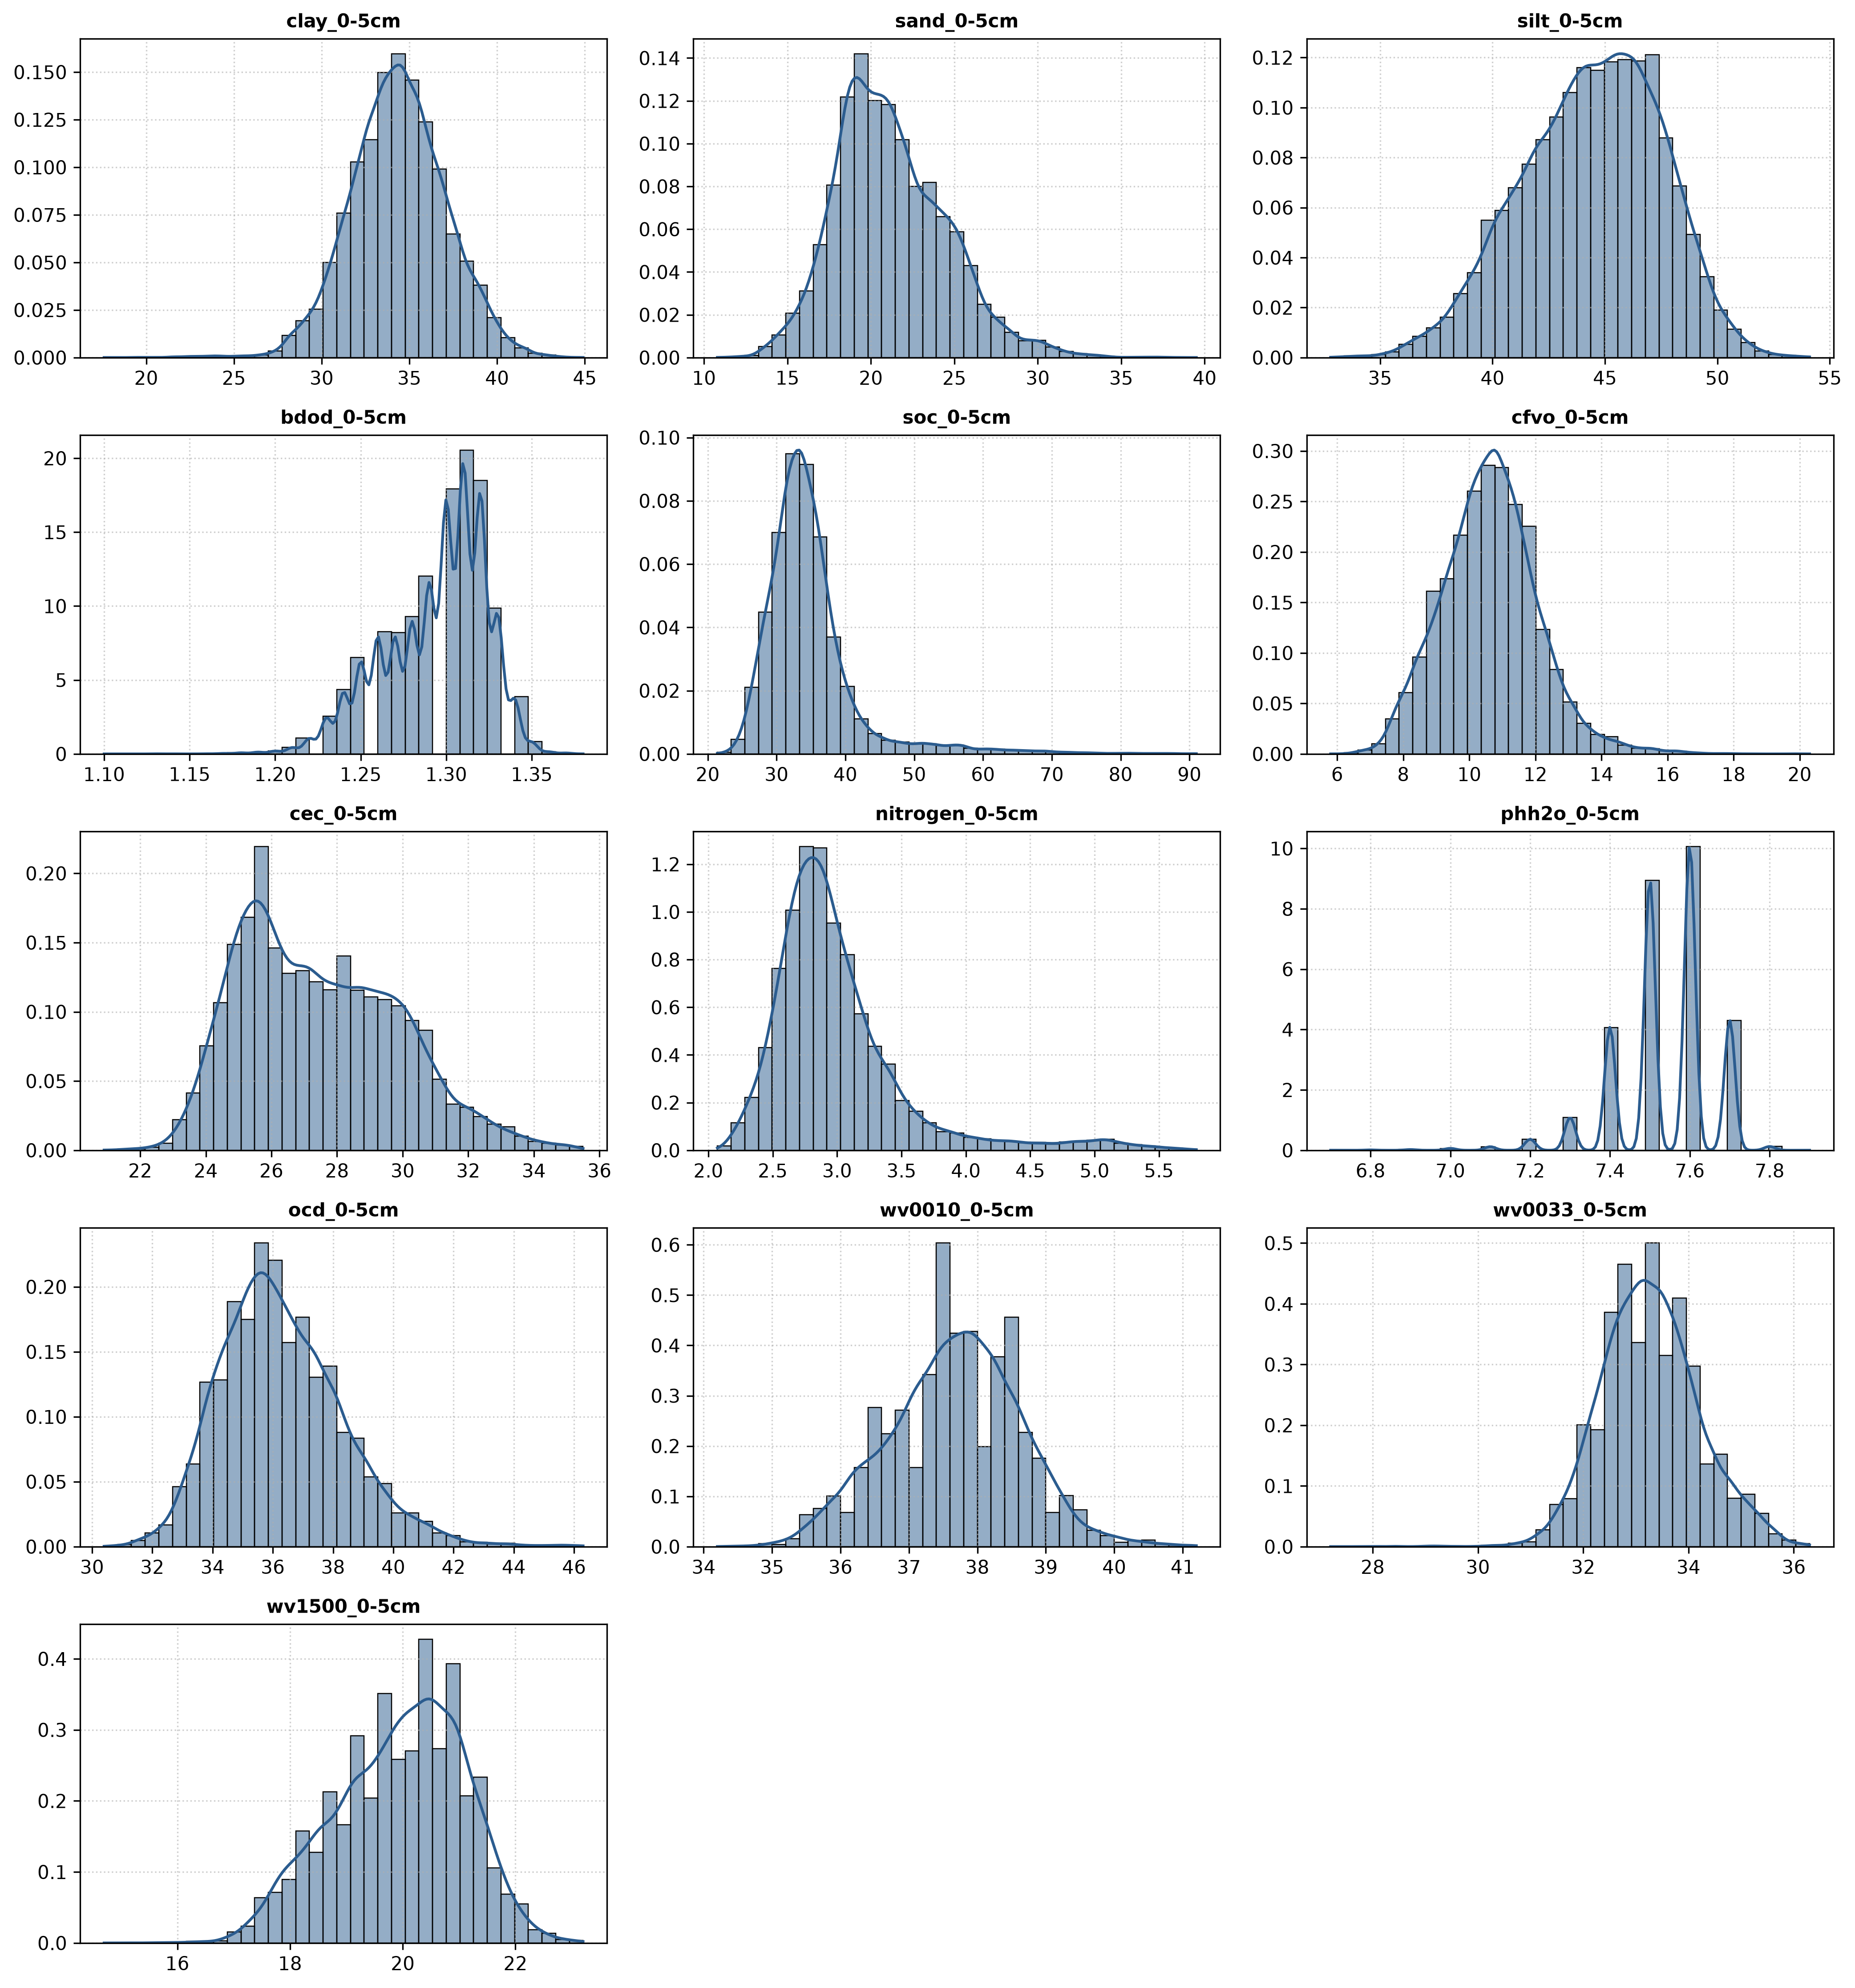
\includegraphics[width=\textwidth]{distribuzioni_eda.png}
    \caption{Distribuzioni delle variabili pedologiche nello strato
    superficiale (0--5\,cm). Le curve KDE evidenziano eventuali
    asimmetrie e multimodalità.}
    \label{fig:distribuzioni}
\end{figure}

\subsection{Matrice di Correlazione}

La matrice di correlazione completa (Figura~\ref{fig:correlazione}) ha
evidenziato le relazioni attese tra le variabili:

\begin{itemize}
    \item Correlazione \textbf{positiva forte} tra \texttt{soc} e
    \texttt{cec}: la sostanza organica contribuisce significativamente
    alla capacità di scambio cationico.

    \item Correlazione \textbf{negativa} tra \texttt{clay} e
    \texttt{sand}: la complementarietà granulometrica.

    \item Correlazione \textbf{positiva} tra le variabili idriche
    (\texttt{wv0010}, \texttt{wv0033}, \texttt{wv1500}): coerenza
    della ritenzione idrica.
\end{itemize}

\begin{figure}[H]
    \centering
    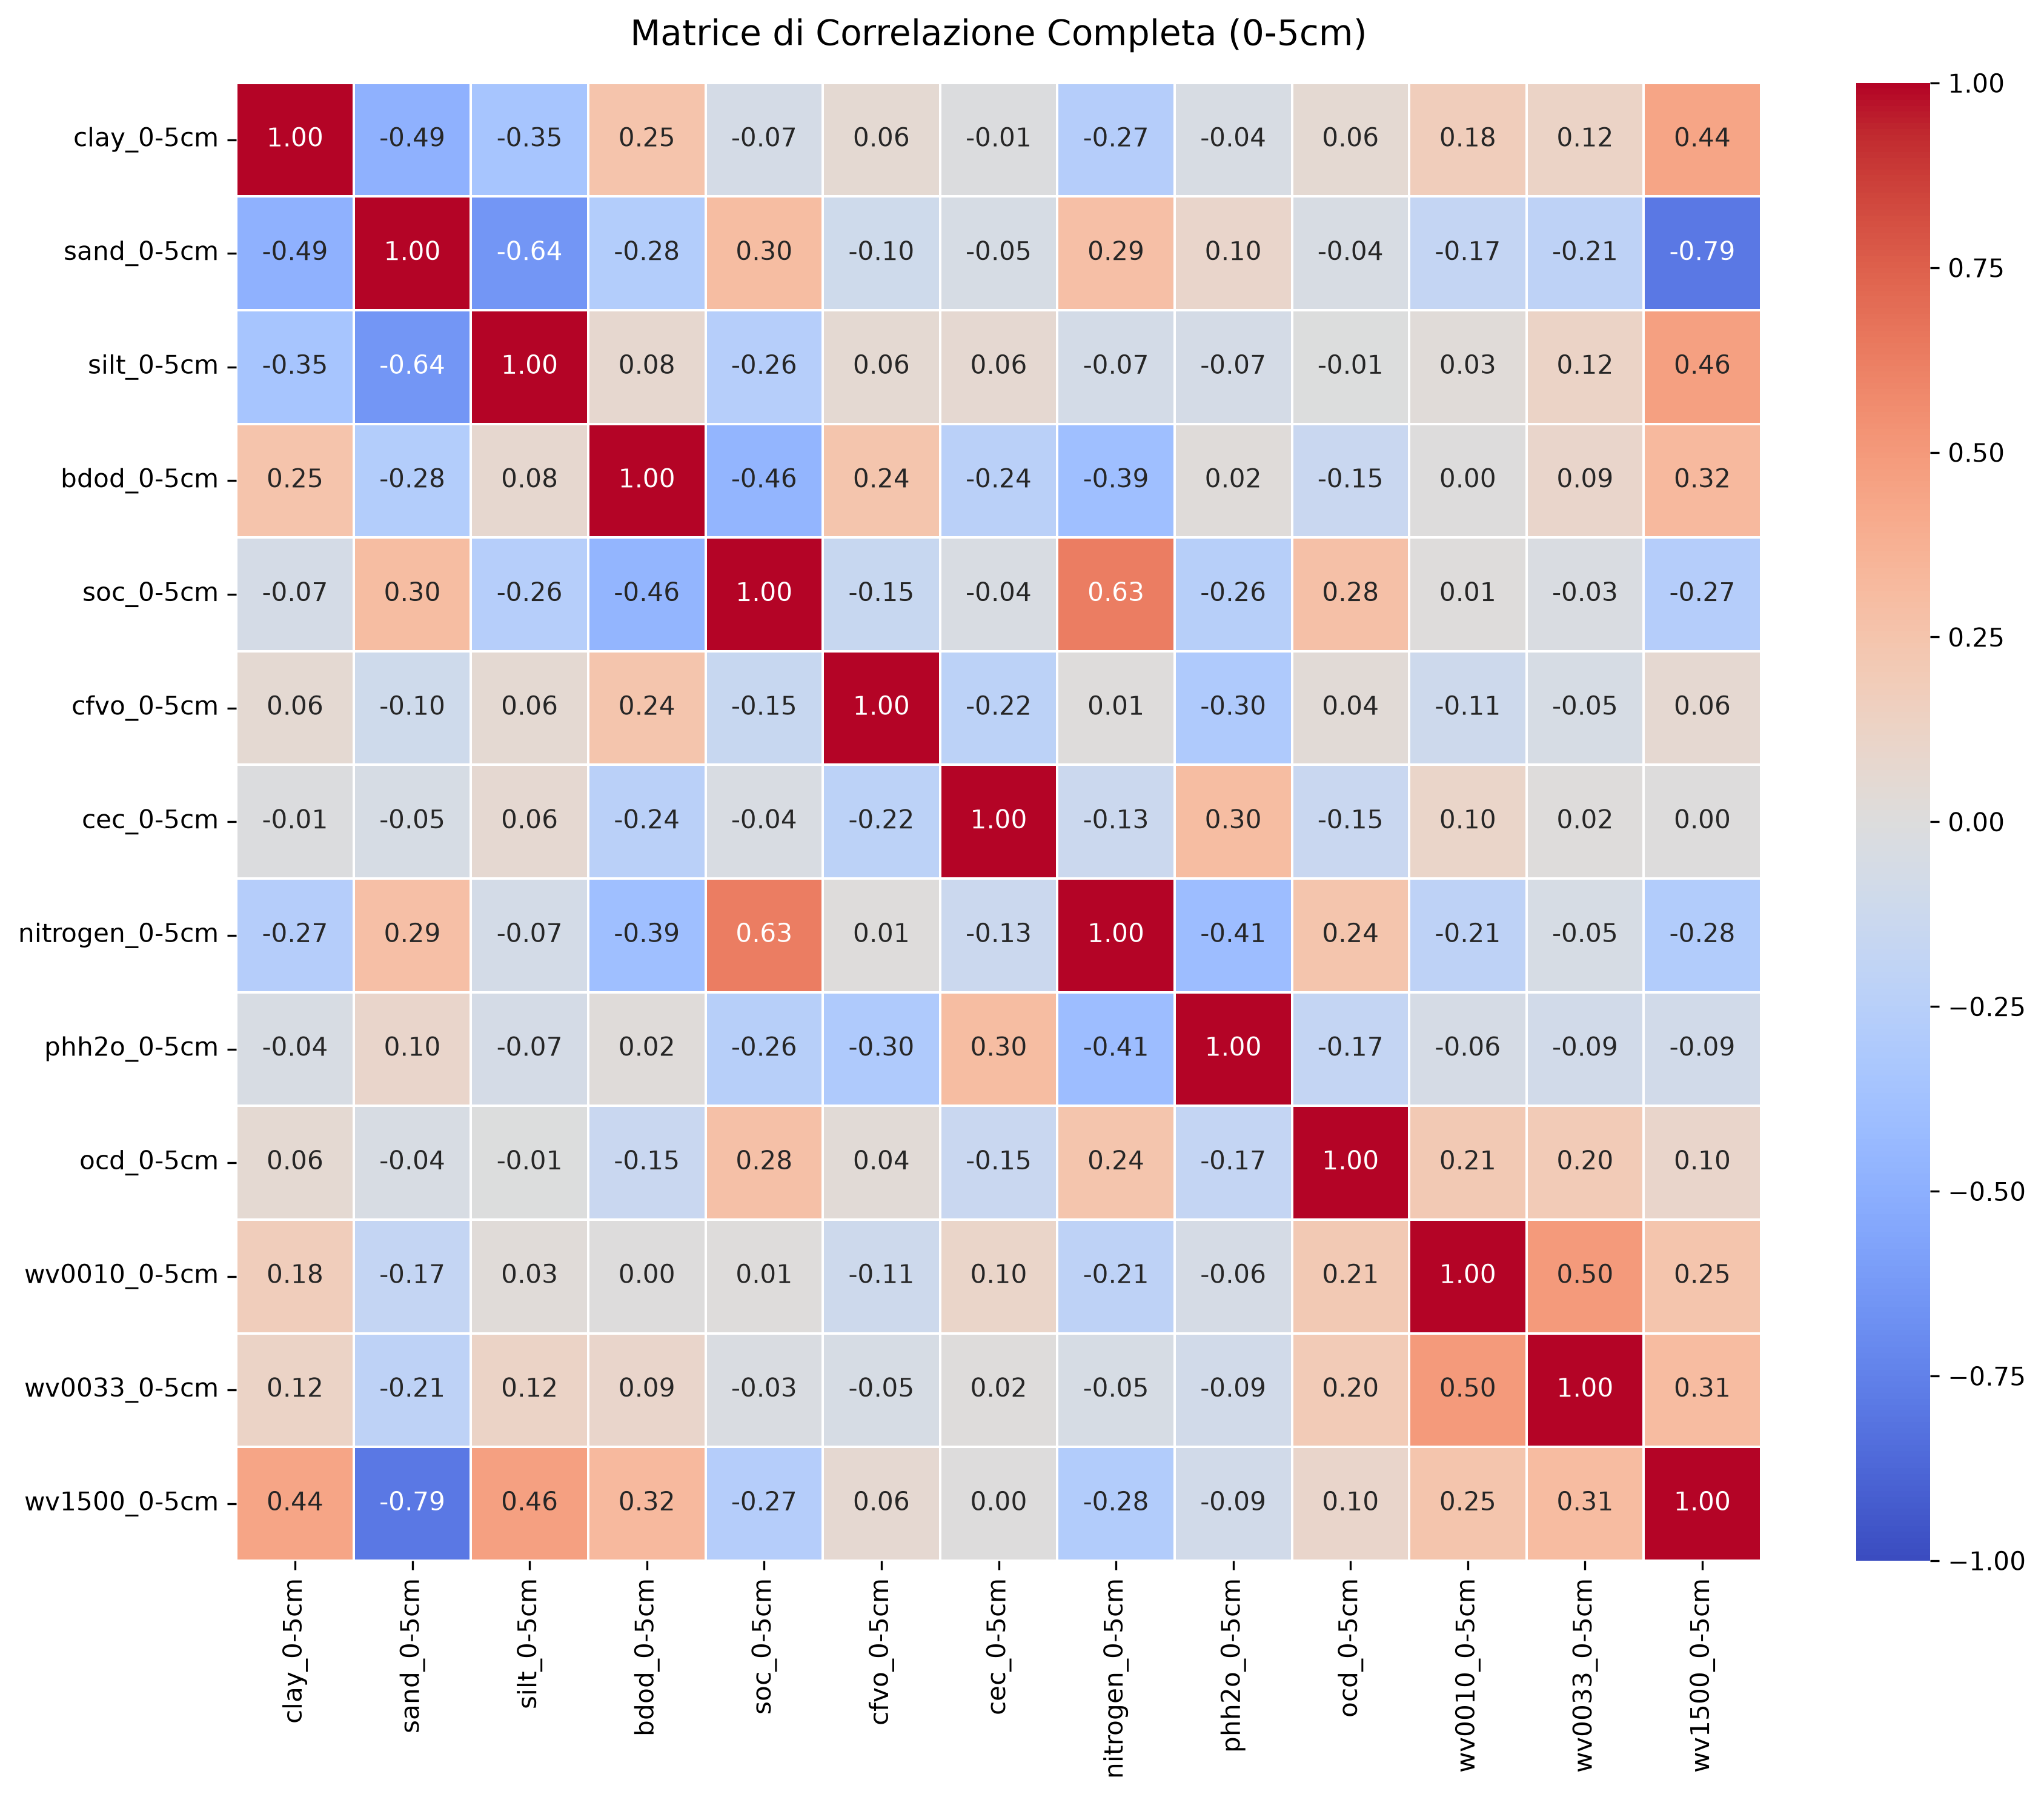
\includegraphics[width=0.85\textwidth]{matrice_correlazione.png}
    \caption{Matrice di correlazione delle variabili pedologiche
    superficiali. I valori numerici sono annotati nella heatmap
    \texttt{coolwarm}.}
    \label{fig:correlazione}
\end{figure}


% ══════════════════════════════════════════════════════════════════════════
\section{Feature Engineering: Gradienti Verticali}
\label{sec:feat_eng}
% ══════════════════════════════════════════════════════════════════════════

\subsection{Motivazione}

Un clustering basato sulle sole variabili superficiali cattura solo
un'istantanea bidimensionale del suolo. Per cogliere la complessità del
profilo pedologico, è necessario descrivere \emph{come} le proprietà
cambiano con la profondità. A tal fine, sono stati calcolati i
\textbf{gradienti normalizzati} tra strati consecutivi.

\subsection{Gradienti Normalizzati}

Il \textbf{gradiente normalizzato} quantifica il tasso di variazione tra
due strati consecutivi, normalizzato per la distanza (in cm) tra i
centri degli strati:

\begin{equation}
    g^{(v)}_{i \to i+1} = \frac{X^{(v)}_{d_{i+1}} - X^{(v)}_{d_i}}
    {z_{i+1} - z_i}
    \label{eq:gradiente}
\end{equation}

dove $z_i$ e $z_{i+1}$ sono i punti medi (in cm) dei due strati. I
punti medi utilizzati sono: 2.5, 10.0, 22.5, 45.0, 80.0 e 150.0\,cm
(Tabella~\ref{tab:midpoints}).

\begin{table}[H]
    \centering
    \caption{Punti medi degli strati di profondità SoilGrids.}
    \label{tab:midpoints}
    \begin{tabular}{@{}lc@{}}
        \toprule
        \textbf{Strato} & \textbf{Punto medio (cm)} \\
        \midrule
        0--5\,cm    & 2.5   \\
        5--15\,cm   & 10.0  \\
        15--30\,cm  & 22.5  \\
        30--60\,cm  & 45.0  \\
        60--100\,cm & 80.0  \\
        100--200\,cm & 150.0 \\
        \bottomrule
    \end{tabular}
\end{table}
Questa normalizzazione è fondamentale perché gli strati SoilGrids hanno
spessori diversi (5, 10, 15, 30, 40 e 100\,cm): senza normalizzazione,
il gradiente tra 60--100\,cm e 100--200\,cm (distanza di 70\,cm tra i
centri) non sarebbe comparabile con quello tra 0--5\,cm e 5--15\,cm
(distanza di 7.5\,cm).

\begin{lstlisting}[caption={Calcolo dei gradienti normalizzati tra strati consecutivi.},label={lst:gradient}]
layer_midpoints = {
    '0-5cm': 2.5, '5-15cm': 10.0, '15-30cm': 22.5,
    '30-60cm': 45.0, '60-100cm': 80.0, '100-200cm': 150.0
}

def calc_gradient(da, l_top, l_bottom):
    dz = layer_midpoints[l_bottom] - layer_midpoints[l_top]
    return (da.sel(depth=l_bottom) - da.sel(depth=l_top)) / dz
\end{lstlisting}

\subsection{Selezione delle 13 Feature Finali}

Dopo il calcolo, sono state selezionate 13 feature suddivise
in sei gruppi tematici (Tabella~\ref{tab:feature}). Ogni gradiente
è stato scelto per catturare una specifica dinamica pedologica lungo
il profilo verticale. Oltre alle variabili
pedologiche classiche, è stata inclusa la \textbf{conduttività idraulica
saturata} (\texttt{Ksat}), già presente nel dataset NetCDF in quanto
derivata mediante funzioni di pedotrasferimento a partire dalle
variabili tessiturali e idrologiche.

\begin{table}[H]
    \centering
    \caption{Le 13 feature selezionate per il clustering, raggruppate
    per tipologia pedologica.}
    \label{tab:feature}
    \small
    \begin{tabular}{@{}lll@{}}
        \toprule
        \textbf{Gruppo} & \textbf{Feature} & \textbf{Interpretazione} \\
        \midrule
        \multirow{3}{*}{\rotatebox[origin=c]{90}{\textbf{Argilla}}}
        & \texttt{clay\_grad\_0-5\_to\_5-15}     & Dinamica tessiturale superficiale \\
        & \texttt{clay\_grad\_5-15\_to\_15-30}    & Inizio lisciviazione argilla \\
        & \texttt{clay\_grad\_15-30\_to\_30-60}   & Orizzonte argillico (Bt) \\
        \midrule
        \multirow{1}{*}{\textbf{Sabbia}}
        & \texttt{sand\_grad\_30-60\_to\_60-100}  & Discontinuità sedimentarie \\
        \midrule
        \multirow{2}{*}{\rotatebox[origin=c]{90}{\textbf{Scheletro}}}
        & \texttt{cfvo\_grad\_15-30\_to\_30-60}   & Transizioni litologiche \\
        & \texttt{cfvo\_grad\_60-100\_to\_100-200} & Contatto con roccia madre \\
        \midrule
        \multirow{2}{*}{\rotatebox[origin=c]{90}{\textbf{SOC}}}
        & \texttt{soc\_grad\_0-5\_to\_5-15}      & Crollo iniziale sost.\ organica \\
        & \texttt{soc\_grad\_5-15\_to\_15-30}     & Esaurimento zona radicale \\
        \midrule
        \multirow{3}{*}{\rotatebox[origin=c]{90}{\textbf{BDOD}}}
        & \texttt{bdod\_grad\_5-15\_to\_15-30}    & Suola di aratura \\
        & \texttt{bdod\_grad\_15-30\_to\_30-60}   & Compattazione profonda \\
        & \texttt{bdod\_grad\_30-60\_to\_60-100}  & Transizione substrato \\
        \midrule
        \multirow{2}{*}{\rotatebox[origin=c]{90}{\textbf{Ksat}}}
        & \texttt{Ksat\_grad\_0-5\_to\_5-15}      & Variazione drenaggio superficiale \\
        & \texttt{Ksat\_grad\_15-30\_to\_30-60}   & Variazione drenaggio profondo \\
        \bottomrule
    \end{tabular}
\end{table}

\subsection{Analisi di Correlazione delle Feature Ingegnerizzate}

Le correlazioni tra le 13 feature ingegnerizzate sono state analizzate
mediante la matrice di correlazione di Pearson
(Figura~\ref{fig:corr_gradienti}). Un controllo automatico ha verificato
l'assenza di coppie con collinearità critica ($|r| > 0.8$), confermando
che lo spazio delle feature è ben bilanciato e non richiede ulteriore
riduzione dimensionale.

Le correlazioni osservate confermano le attese pedologiche:
\begin{itemize}
    \item Correlazione \textbf{negativa} tra i gradienti di SOC e i
    gradienti di BDOD: dove la sostanza organica cala rapidamente,
    la densità apparente aumenta.

    \item Correlazione \textbf{negativa} tra i gradienti di argilla e
    il gradiente di sabbia: la complementarietà tessiturale è preservata
    anche nelle dinamiche verticali.

    \item I gradienti di Ksat riflettono indirettamente le dinamiche
    tessiturali, con correlazioni coerenti rispetto ai gradienti di
    argilla e BDOD.
\end{itemize}

\begin{figure}[H]
    \centering
    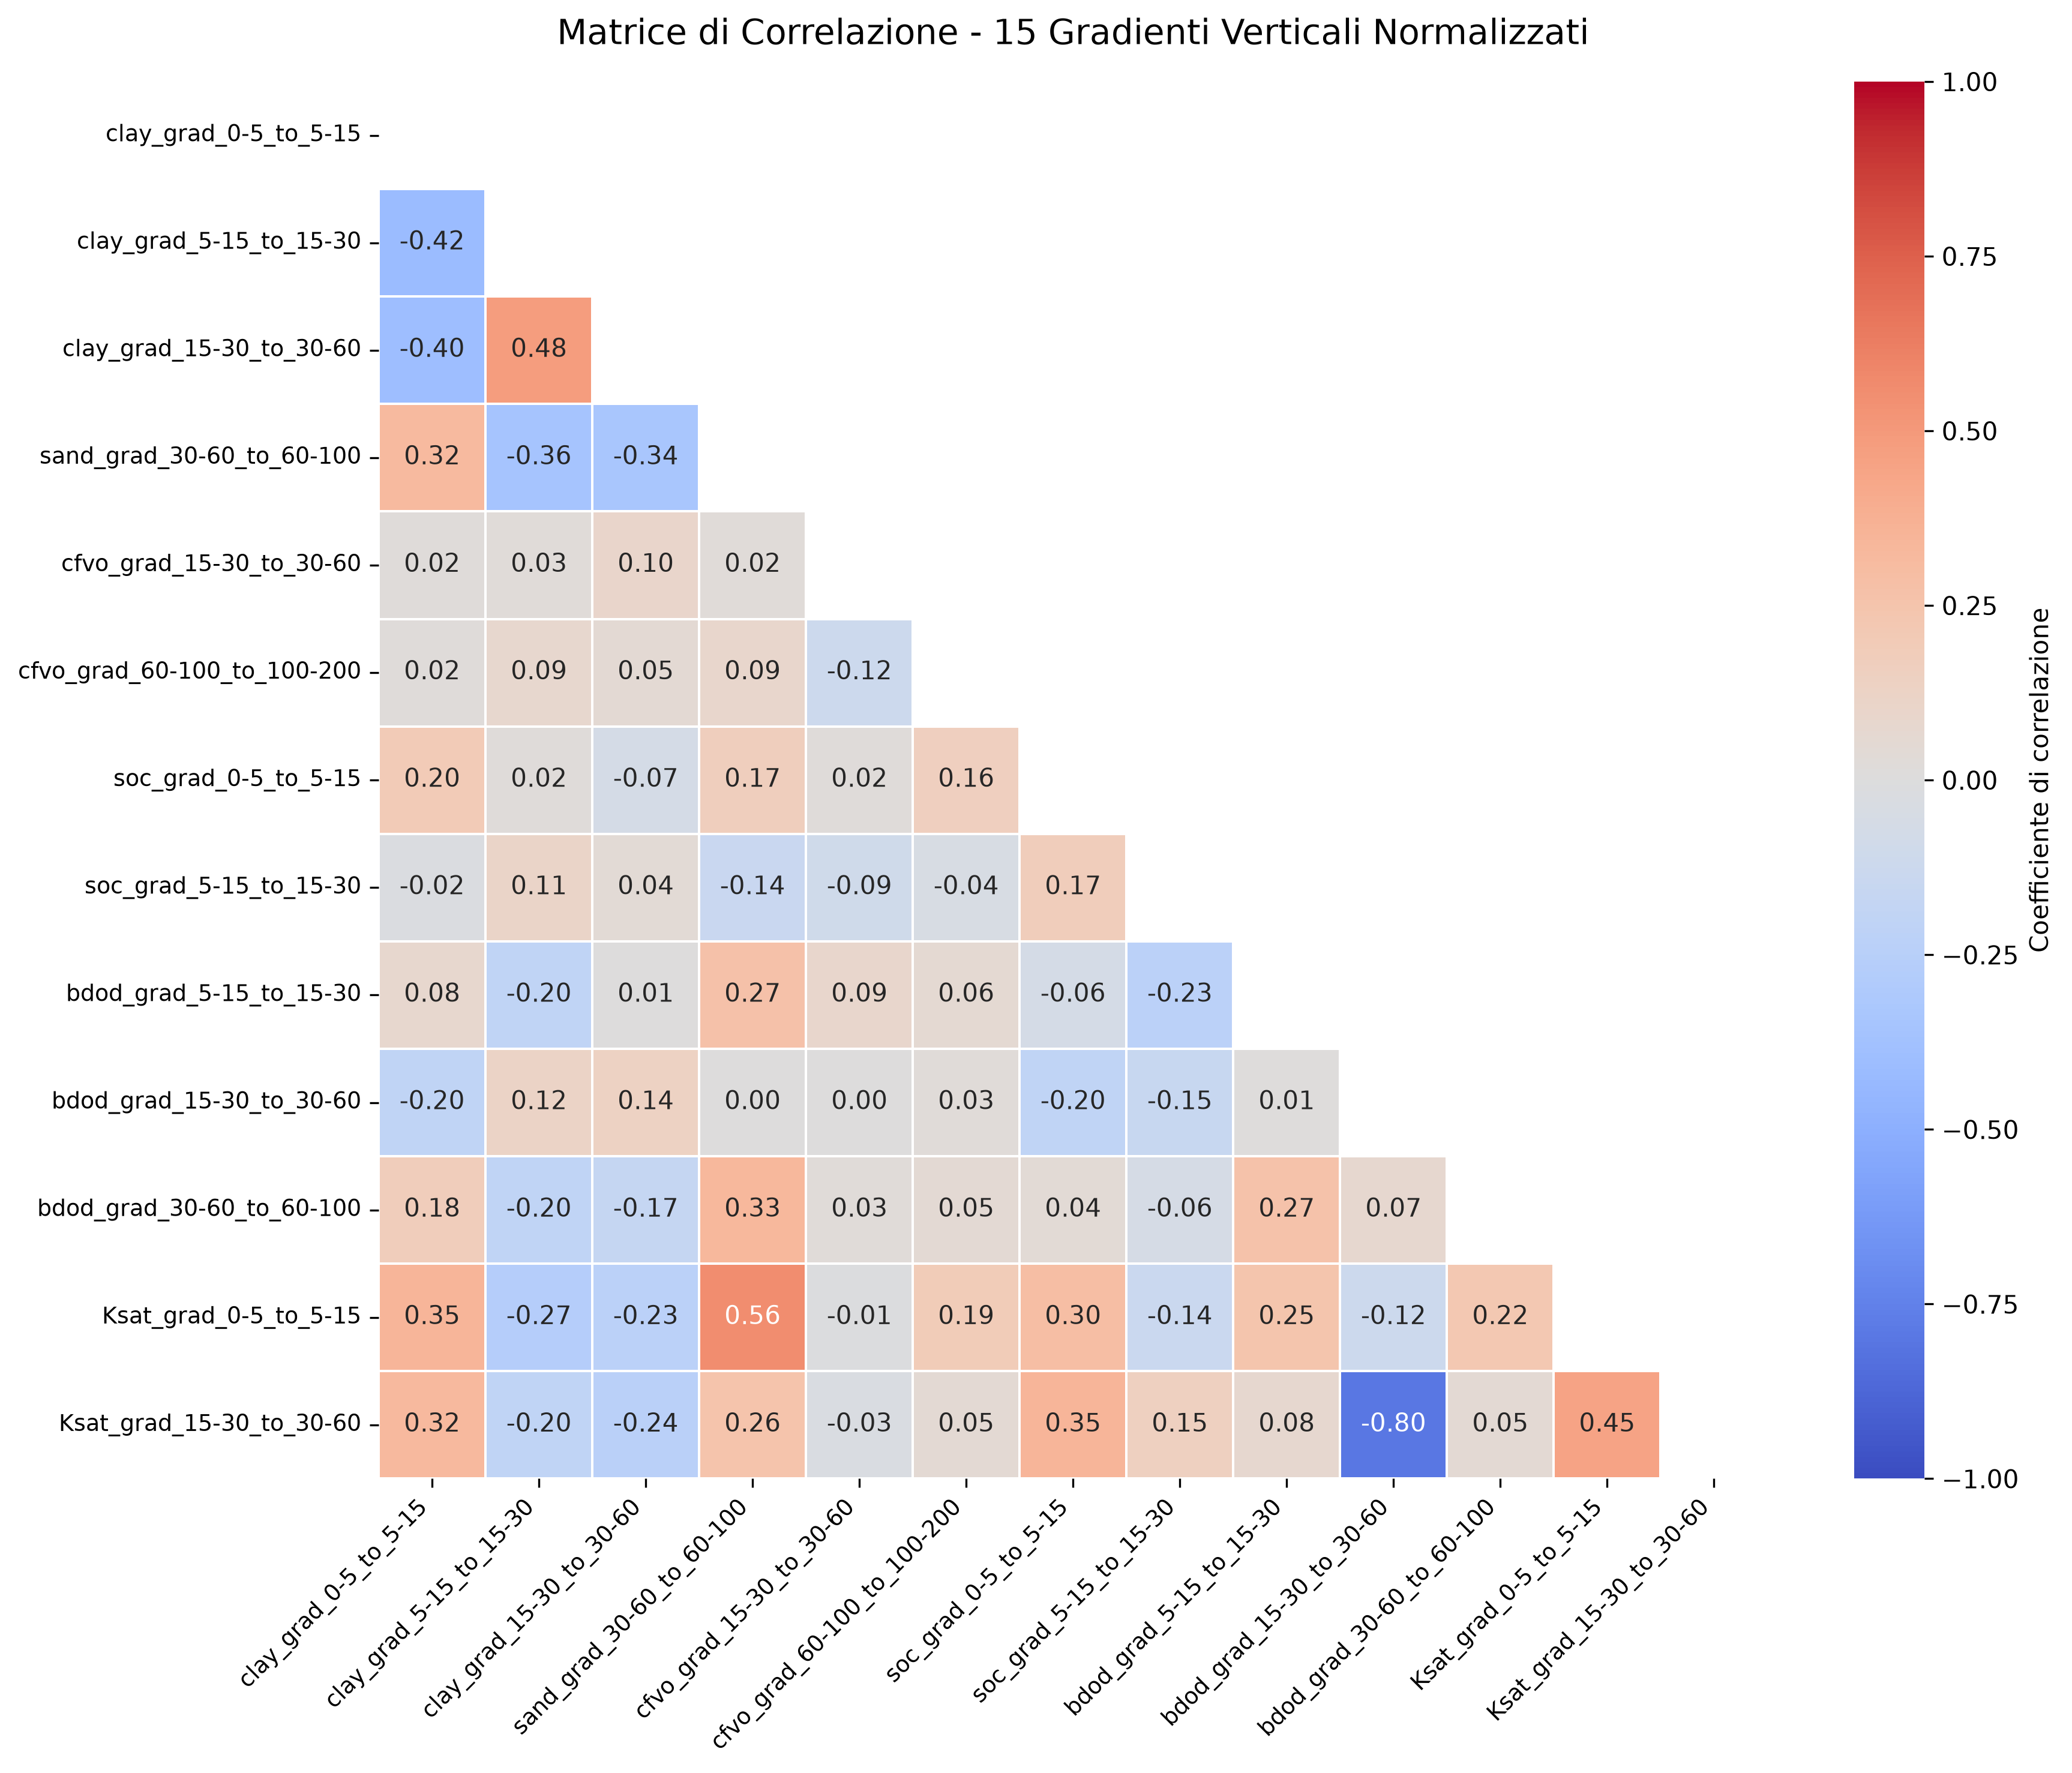
\includegraphics[width=0.85\textwidth]{corr_deep.png}
    \caption{Matrice di correlazione (triangolo inferiore) dei 13
    gradienti verticali normalizzati. Nessuna coppia supera la soglia
    critica $|r| > 0.8$.}
    \label{fig:corr_gradienti}
\end{figure}


% ══════════════════════════════════════════════════════════════════════════
\section{Metodologia}
\label{sec:metodologia}
% ══════════════════════════════════════════════════════════════════════════

\subsection{Standardizzazione dei Dati}

Le 13 feature selezionate presentano scale e deviazioni standard molto
diverse. Per evitare che le variabili a scala maggiore dominino
il calcolo delle distanze euclidee, è stato applicato uno
\textbf{StandardScaler}:

\begin{equation}
    \tilde{x}_j = \frac{x_j - \mu_j}{\sigma_j}
    \label{eq:scaler}
\end{equation}

dove $\mu_j$ e $\sigma_j$ sono rispettivamente la media e la deviazione
standard della $j$-esima feature sul dataset completo.

\subsection{Campionamento per Ottimizzazione}

Per rendere computazionalmente fattibile la ricerca degli iperparametri
(in particolare il calcolo del Coefficiente di Silhouette, che ha
complessità $O(n^2)$), è stato estratto un campione casuale
di \textbf{15\,000 pixel} dal dataset standardizzato.

\subsection{Algoritmo 1: K-Means}

L'algoritmo \kmeans{} partiziona $n$ osservazioni in $K$ cluster
minimizzando la \textbf{Sum of Squared Errors} (SSE) intra-cluster:

\begin{equation}
    \text{SSE} = \sum_{k=1}^{K} \sum_{\mathbf{x}_i \in C_k}
    \|\mathbf{x}_i - \boldsymbol{\mu}_k\|^2
    \label{eq:sse}
\end{equation}

dove $\boldsymbol{\mu}_k$ è il centroide del cluster $C_k$.
L'inizializzazione dei centroidi è stata effettuata con la strategia
\textbf{k-means++}, che seleziona i centri iniziali in modo da
massimizzare la distanza reciproca, garantendo una convergenza più
rapida e stabile.

\subsubsection{Ricerca del K Ottimale}

La determinazione del numero ottimale di cluster è stata affrontata con
quattro metriche complementari, calcolate per $K \in [2, 12]$:

\begin{enumerate}
    \item \textbf{Metodo del Gomito (Inerzia)}: la curva di inerzia
    (SSE) al variare di $K$ viene analizzata con l'algoritmo
    \texttt{KneeLocator} della libreria \texttt{kneed}, che individua
    automaticamente il punto di flesso geometrico (``gomito'') nella
    curva convessa decrescente.

    \item \textbf{Coefficiente di Silhouette}: misura la coesione
    intra-cluster e la separazione inter-cluster (cfr.\
    Sezione~\ref{subsec:metriche}). Il $K$ con il valore massimo è
    selezionato.

    \item \textbf{Indice di Davies-Bouldin (DB)}: valuta la somiglianza
    tra cluster adiacenti. Definito come:
    \begin{equation}
        \text{DB} = \frac{1}{K} \sum_{k=1}^{K} \max_{j \neq k}
        \left( \frac{s_k + s_j}{d_{kj}} \right)
    \end{equation}
    dove $s_k$ è la dispersione media del cluster $k$ e $d_{kj}$ la
    distanza tra i centroidi $k$ e $j$. Un valore \textbf{più basso}
    indica cluster meglio separati.

    \item \textbf{Indice di Calinski-Harabasz (CH)}: rapporto tra la
    dispersione inter-cluster e intra-cluster, pesato per i gradi di
    libertà:
    \begin{equation}
        \text{CH} = \frac{\text{SSB} / (K-1)}{\text{SSW} / (n-K)}
    \end{equation}
    dove SSB è la varianza inter-cluster e SSW la varianza intra-cluster.
    Un valore \textbf{più alto} indica cluster più compatti e separati.
\end{enumerate}

\begin{lstlisting}[caption={Calcolo delle quattro metriche per la ricerca del K ottimale.},label={lst:metriche_k}]
k_values = list(range(2, 13))
for k in k_values:
    model = KMeans(n_clusters=k, init="k-means++",
                   n_init=10, max_iter=300, random_state=42)
    labels = model.fit_predict(X_search)

    inertia_values.append(model.inertia_)
    silhouette_scores.append(silhouette_score(X_search, labels))
    db_scores.append(davies_bouldin_score(X_search, labels))
    ch_scores.append(calinski_harabasz_score(X_search, labels))

# Individuazione automatica del gomito
kneedle = KneeLocator(k_values, inertia_values,
                       curve="convex", direction="decreasing",
                       interp_method="polynomial")
best_k_elbow = kneedle.elbow
\end{lstlisting}

\subsubsection{Scelta Finale: K=6}

I risultati delle quattro metriche (Tabella~\ref{tab:kottimale}) sono
stati analizzati congiuntamente. Sebbene metriche come la Silhouette e
il Davies-Bouldin tendano a favorire valori bassi di $K$ (ad esempio
$K=2$), producendo una separazione binaria del territorio priva di
sfumature agronomiche, il Metodo del Gomito ha indicato un punto di
flesso coerente con $K=6$.

La scelta finale di \kval{6} è stata guidata da un bilanciamento tra
i criteri statistici e le considerazioni pedologiche di dominio:
con sei cluster è possibile distinguere tipologie di suolo con
dinamiche verticali distinte (ad esempio, suoli con forte lisciviazione
argillosa vs.\ suoli con profilo uniforme, suoli con suola di
lavorazione vs.\ suoli profondi organici).

\subsection{Algoritmo 2: DBSCAN}

Il \textbf{DBSCAN} (Density-Based Spatial Clustering of Applications
with Noise) identifica cluster come regioni ad alta densità separate da
regioni a bassa densità, classificando come \emph{rumore} ($-1$) i
punti isolati.

Due sono i parametri chiave:
\begin{itemize}
    \item $\varepsilon$ (\texttt{eps}): raggio massimo del vicinato.
    \item \texttt{min\_samples}: numero minimo di punti per formare un
    nucleo denso.
\end{itemize}

Il parametro \texttt{min\_samples} è stato fissato a 26
($\approx 2 \times d$, con $d = 13$ il numero di feature), seguendo
le linee guida per dati ad alta dimensionalità. La determinazione di
$\varepsilon$ è stata effettuata tramite il \textbf{grafico K-NN
distance}: calcolando la distanza dal $k$-esimo vicino più prossimo
(con $k = 26$) e ordinando i valori in modo crescente, si individua
il punto di ginocchio che segna il passaggio da ``densità
intra-cluster'' a ``distanza inter-cluster''. Il valore scelto è stato
$\varepsilon = 1.9$: l'euristica del metodo del gomito avrebbe dato $\varepsilon \approx 2.6$, ma con tale valore l'intero dataset sarebbe collassato in un singolo cluster senza alcun outlier. 

\begin{figure}[H]
    \centering
    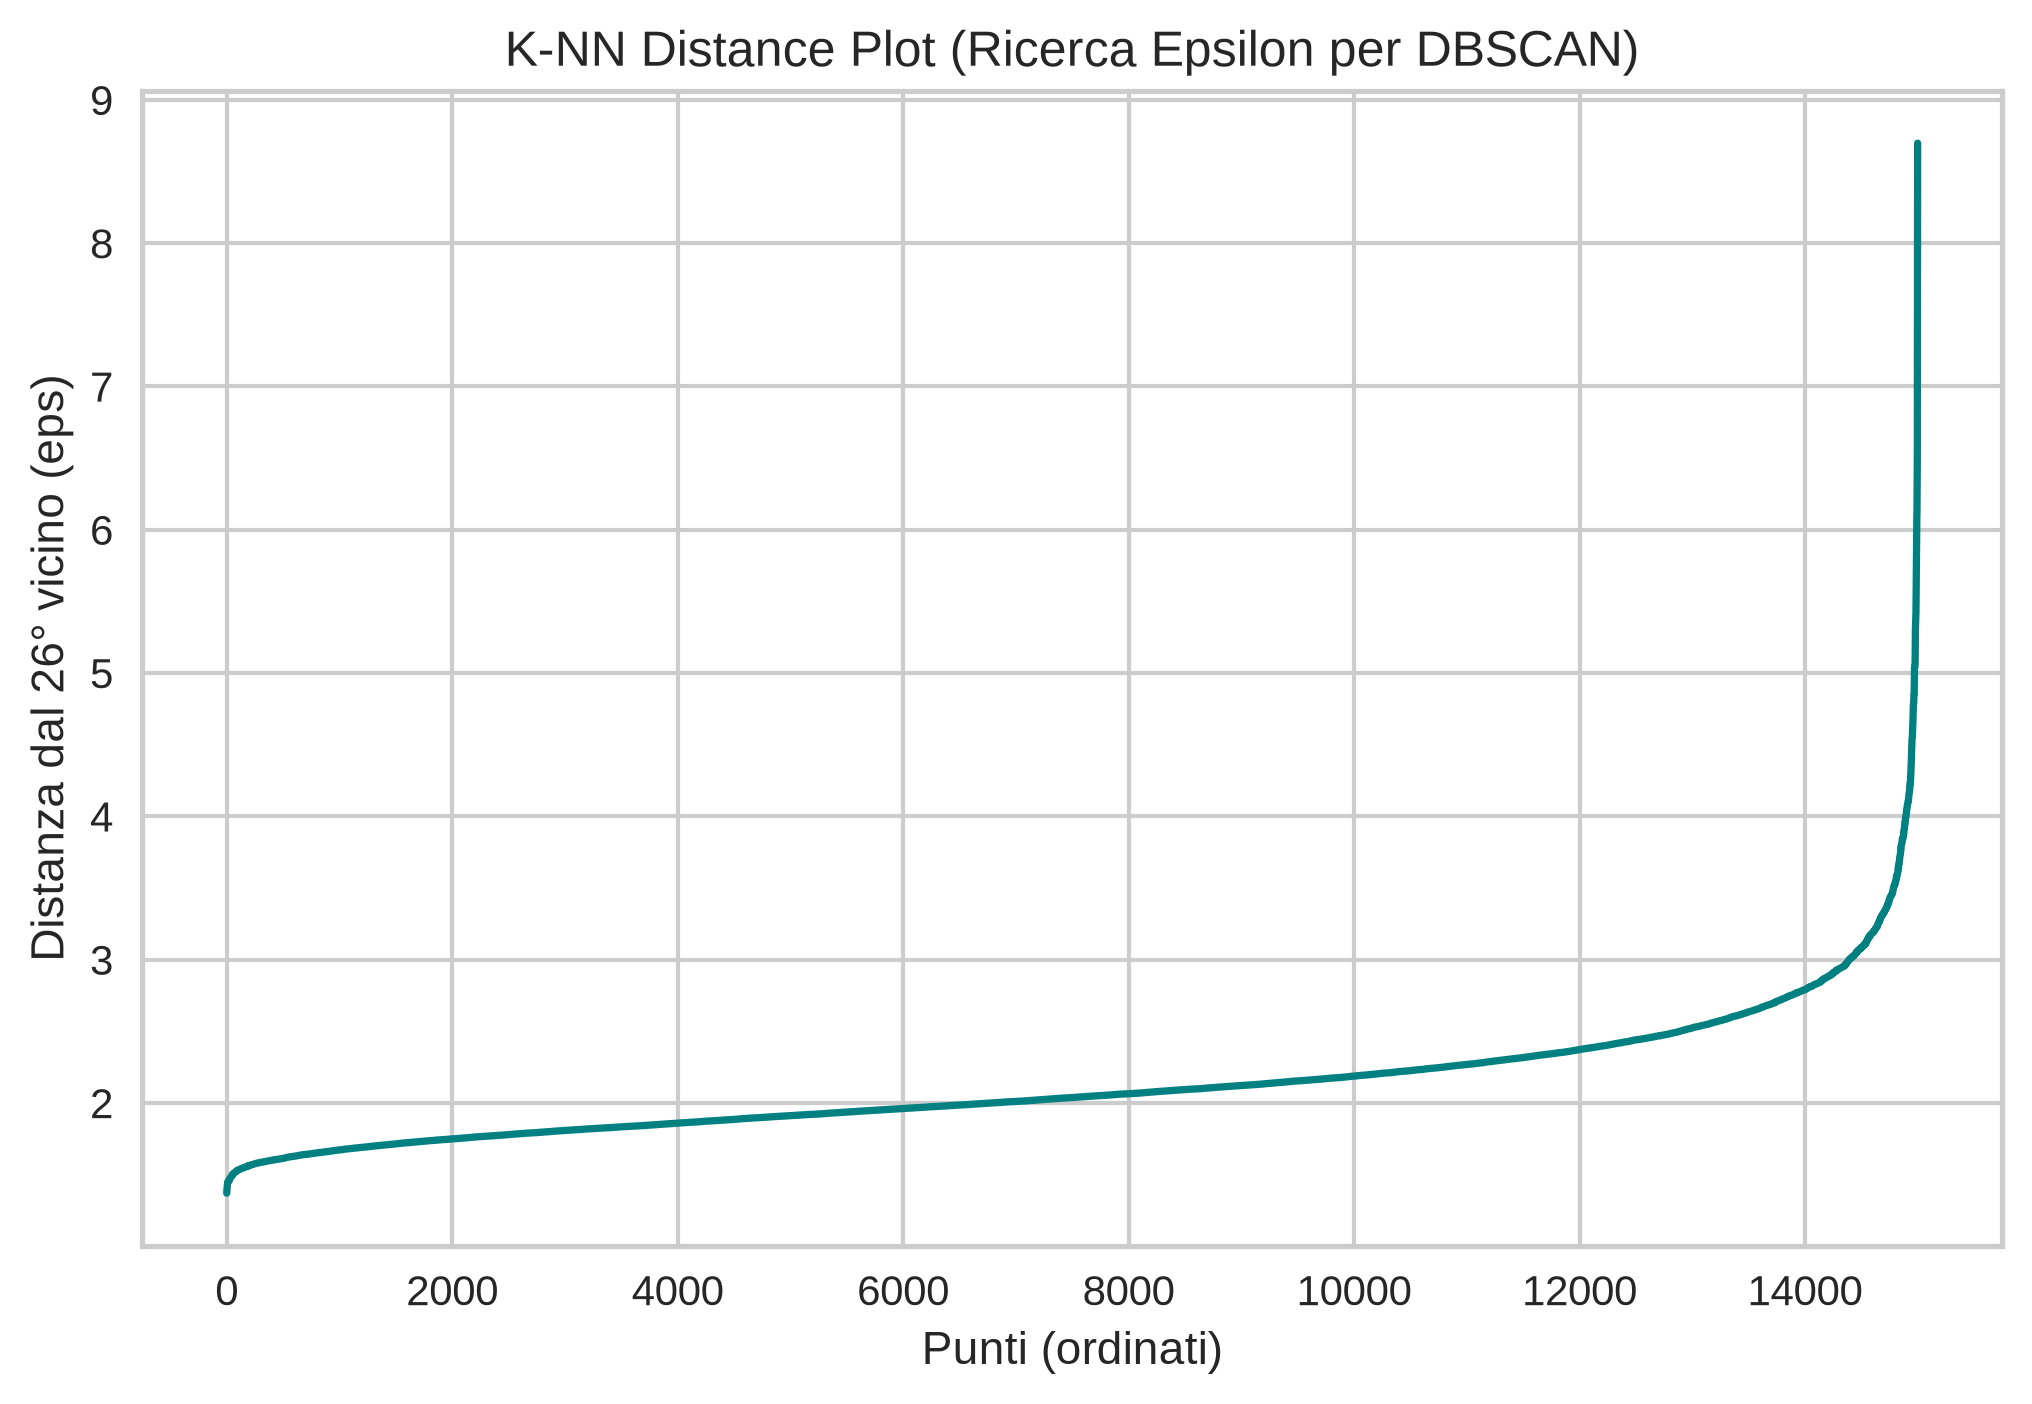
\includegraphics[width=0.65\textwidth]{knn_distance.png}
    \caption{Grafico delle distanze K-NN per la determinazione
    dell'epsilon ottimale del DBSCAN. Il punto di ginocchio è stato
    individuato nella regione $\varepsilon \approx 2.6$.}
    \label{fig:knn}
\end{figure}

\subsection{Algoritmo 3: Bisecting K-Means}

Il \textbf{Bisecting \kmeans{}} è un approccio gerarchico \emph{divisivo}
(top-down): parte da un unico macro-cluster e lo suddivide iterativamente
in due sotto-cluster fino a raggiungere il numero desiderato di partizioni.

A ogni iterazione, il cluster con la varianza interna maggiore viene
selezionato e bipartito con un \kmeans{} a $K=2$. Il processo è stato
configurato con $K=6$ per garantire un confronto equo con il \kmeans{}
standard.

Per rendere il confronto visivo immediato, le etichette dei cluster
generati dal Bisecting \kmeans{} sono state \textbf{allineate} a quelle
del \kmeans{} standard mediante l'algoritmo ungherese
(\texttt{linear\_sum\_assignment} sulla matrice di confusione),
minimizzando la discrepanza complessiva tra le due partizioni.

\subsection{Algoritmo 4: Gaussian Mixture Model (EM)}
\label{subsec:gmm}

Il \textbf{Gaussian Mixture Model} (GMM) generalizza il \kmeans{} in
ambito probabilistico, modellando i dati come una miscela di $K$
distribuzioni gaussiane multivariate:

\begin{equation}
    p(\mathbf{x}) = \sum_{k=1}^{K} \pi_k \;\mathcal{N}(\mathbf{x}
    \mid \boldsymbol{\mu}_k, \boldsymbol{\Sigma}_k)
    \label{eq:gmm}
\end{equation}

dove $\pi_k$ sono i pesi di miscelazione ($\sum_k \pi_k = 1$),
$\boldsymbol{\mu}_k$ e $\boldsymbol{\Sigma}_k$ sono la media e la
matrice di covarianza della $k$-esima componente gaussiana.

I parametri vengono stimati mediante l'algoritmo iterativo
\textbf{Expectation-Maximization (EM)}:

\begin{enumerate}
    \item \textbf{E-step (Expectation)}: per ogni campione $\mathbf{x}_i$,
    si calcola la \emph{responsabilità} $\gamma_{ik}$, ovvero la
    probabilità a posteriori che $\mathbf{x}_i$ appartenga alla componente
    $k$:
    \begin{equation}
        \gamma_{ik} = \frac{\pi_k \;\mathcal{N}(\mathbf{x}_i \mid
        \boldsymbol{\mu}_k, \boldsymbol{\Sigma}_k)}
        {\sum_{j=1}^{K} \pi_j \;\mathcal{N}(\mathbf{x}_i \mid
        \boldsymbol{\mu}_j, \boldsymbol{\Sigma}_j)}
    \end{equation}

    \item \textbf{M-step (Maximization)}: si aggiornano i parametri di
    ogni componente usando le responsabilità come pesi:
    \begin{align}
        \boldsymbol{\mu}_k^{\text{new}} &= \frac{\sum_i \gamma_{ik}
        \mathbf{x}_i}{\sum_i \gamma_{ik}} \\
        \boldsymbol{\Sigma}_k^{\text{new}} &= \frac{\sum_i \gamma_{ik}
        (\mathbf{x}_i - \boldsymbol{\mu}_k^{\text{new}})
        (\mathbf{x}_i - \boldsymbol{\mu}_k^{\text{new}})^\top}
        {\sum_i \gamma_{ik}} \\
        \pi_k^{\text{new}} &= \frac{1}{n} \sum_i \gamma_{ik}
    \end{align}
\end{enumerate}

L'iterazione prosegue fino a convergenza della log-verosimiglianza.
Rispetto al \kmeans{}, il GMM offre due vantaggi fondamentali:

\begin{itemize}
    \item \textbf{Assegnazione probabilistica} (\emph{soft clustering}):
    ogni pixel riceve una probabilità di appartenenza a ciascun cluster,
    piuttosto che un'assegnazione deterministica. Questo è
    particolarmente utile in pedologia, dove le transizioni tra tipi di
    suolo sono graduali.

    \item \textbf{Cluster ellissoidali}: la matrice di covarianza
    completa consente di modellare cluster non sferici, catturando
    correlazioni tra le feature.
\end{itemize}

Per la selezione del numero ottimale di componenti, sono stati utilizzati
il \textbf{Bayesian Information Criterion (BIC)} e l'\textbf{Akaike
Information Criterion (AIC)}:

\begin{align}
    \text{BIC} &= -2 \ln \hat{L} + p \ln n \\
    \text{AIC} &= -2 \ln \hat{L} + 2p
\end{align}

dove $\hat{L}$ è la verosimiglianza massimizzata, $p$ il numero di
parametri liberi e $n$ la dimensione del campione. Entrambi i criteri
penalizzano la complessità del modello, ma il BIC impone una penalità
più severa, tendendo a preferire modelli più parsimoniosi.

Il modello finale è stato configurato con \texttt{covariance\_type='full'}
(matrice di covarianza completa per ogni componente) e $K=6$ per
consentire un confronto equo con gli altri algoritmi.

\subsection{Riduzione Dimensionale: PCA}

Per la \textbf{visualizzazione} dei cluster nello spazio delle feature
(13 dimensioni), è stata applicata un'analisi delle Componenti
Principali (PCA) per proiettare i dati in 2D:

\begin{equation}
    \mathbf{z}_i = \mathbf{W}^\top \tilde{\mathbf{x}}_i
\end{equation}

dove $\mathbf{W} \in \mathbb{R}^{13 \times 2}$ è la matrice delle prime
due componenti principali, calcolate come gli autovettori associati ai
due autovalori maggiori della matrice di covarianza.

\subsection{Metriche di Validazione}
\label{subsec:metriche}

La validazione dei modelli è stata condotta con metriche sia interne
(non richiedono etichette ground-truth) che relative (confronto tra
partizioni).

\paragraph{Coefficiente di Silhouette.} Per ogni campione $i$:

\begin{equation}
    s(i) = \frac{b(i) - a(i)}{\max\{a(i),\, b(i)\}}
\end{equation}

dove $a(i)$ è la distanza media intra-cluster e $b(i)$ è la distanza
media al cluster più vicino. Il valore medio $\bar{s} \in [-1, 1]$:
valori prossimi a 1 indicano cluster ben separati.

\textbf{Nota metodologica:} per il DBSCAN, il Coefficiente di Silhouette
è stato calcolato \emph{escludendo} i punti classificati come rumore
(etichetta $-1$). Includere tali punti penalizzerebbe artificialmente
l'algoritmo, poiché i punti di rumore non appartengono ad alcun cluster e
generano valori di silhouette fortemente negativi, distorcendo la media
complessiva.

\paragraph{Sum of Squared Error (SSE / Inerzia).} Definita
nell'Eq.~\eqref{eq:sse}, misura la coesione interna dei cluster. Un
valore più basso indica cluster più compatti. Questa metrica non è
applicabile al DBSCAN né al GMM (che ottimizza la verosimiglianza
anziché l'SSE).

\paragraph{BIC e AIC.} Per il GMM, la selezione del modello è stata
guidata dal BIC e dall'AIC (cfr.\ Sezione~\ref{subsec:gmm}), che bilanciano
bontà del fit e complessità.

\paragraph{Adjusted Rand Index (ARI).} Misura la concordanza tra due
partizioni, corretta per il caso. Assume valori in $[-1, 1]$: un ARI
di 1 indica accordo perfetto, 0 indica concordanza casuale.

\paragraph{Normalized Mutual Information (NMI).} Quantifica
l'informazione condivisa tra due partizioni, normalizzata nell'intervallo
$[0, 1]$. Valori elevati indicano forte accordo strutturale.


% ══════════════════════════════════════════════════════════════════════════
\section{Risultati Sperimentali}
\label{sec:risultati}
% ══════════════════════════════════════════════════════════════════════════

\subsection{Ricerca del K Ottimale}

I risultati delle quattro metriche di validazione interna sono
sintetizzati nella Tabella~\ref{tab:kottimale} e visualizzati nella
Figura~\ref{fig:k_selection}.

\begin{table}[H]
    \centering
    \caption{Riepilogo dei valori di $K$ suggeriti dai quattro metodi.}
    \label{tab:kottimale}
    \begin{tabular}{@{}llc@{}}
        \toprule
        \textbf{Metodo / Metrica} & \textbf{Criterio} & \textbf{K suggerito} \\
        \midrule
        Metodo del Gomito (KneeLocator) & Punto di flesso & 6 \\
        Silhouette Score               & Massimo         & 2 \\
        Davies-Bouldin                  & Minimo          & 11 \\
        Calinski-Harabasz               & Massimo         & 2 \\
        \midrule
        \textbf{K finale (dominio)} & \textbf{Agronomico} & \textbf{6} \\
        \bottomrule
    \end{tabular}

    \vspace{4pt}
    {\footnotesize Il Metodo del Gomito conferma $K=6$ come punto di flesso;
    le metriche Silhouette e CH favoriscono $K=2$ (separazione binaria),
    mentre il DB suggerisce $K=11$ (frammentazione eccessiva).}
\end{table}

\begin{figure}[H]
    \centering
    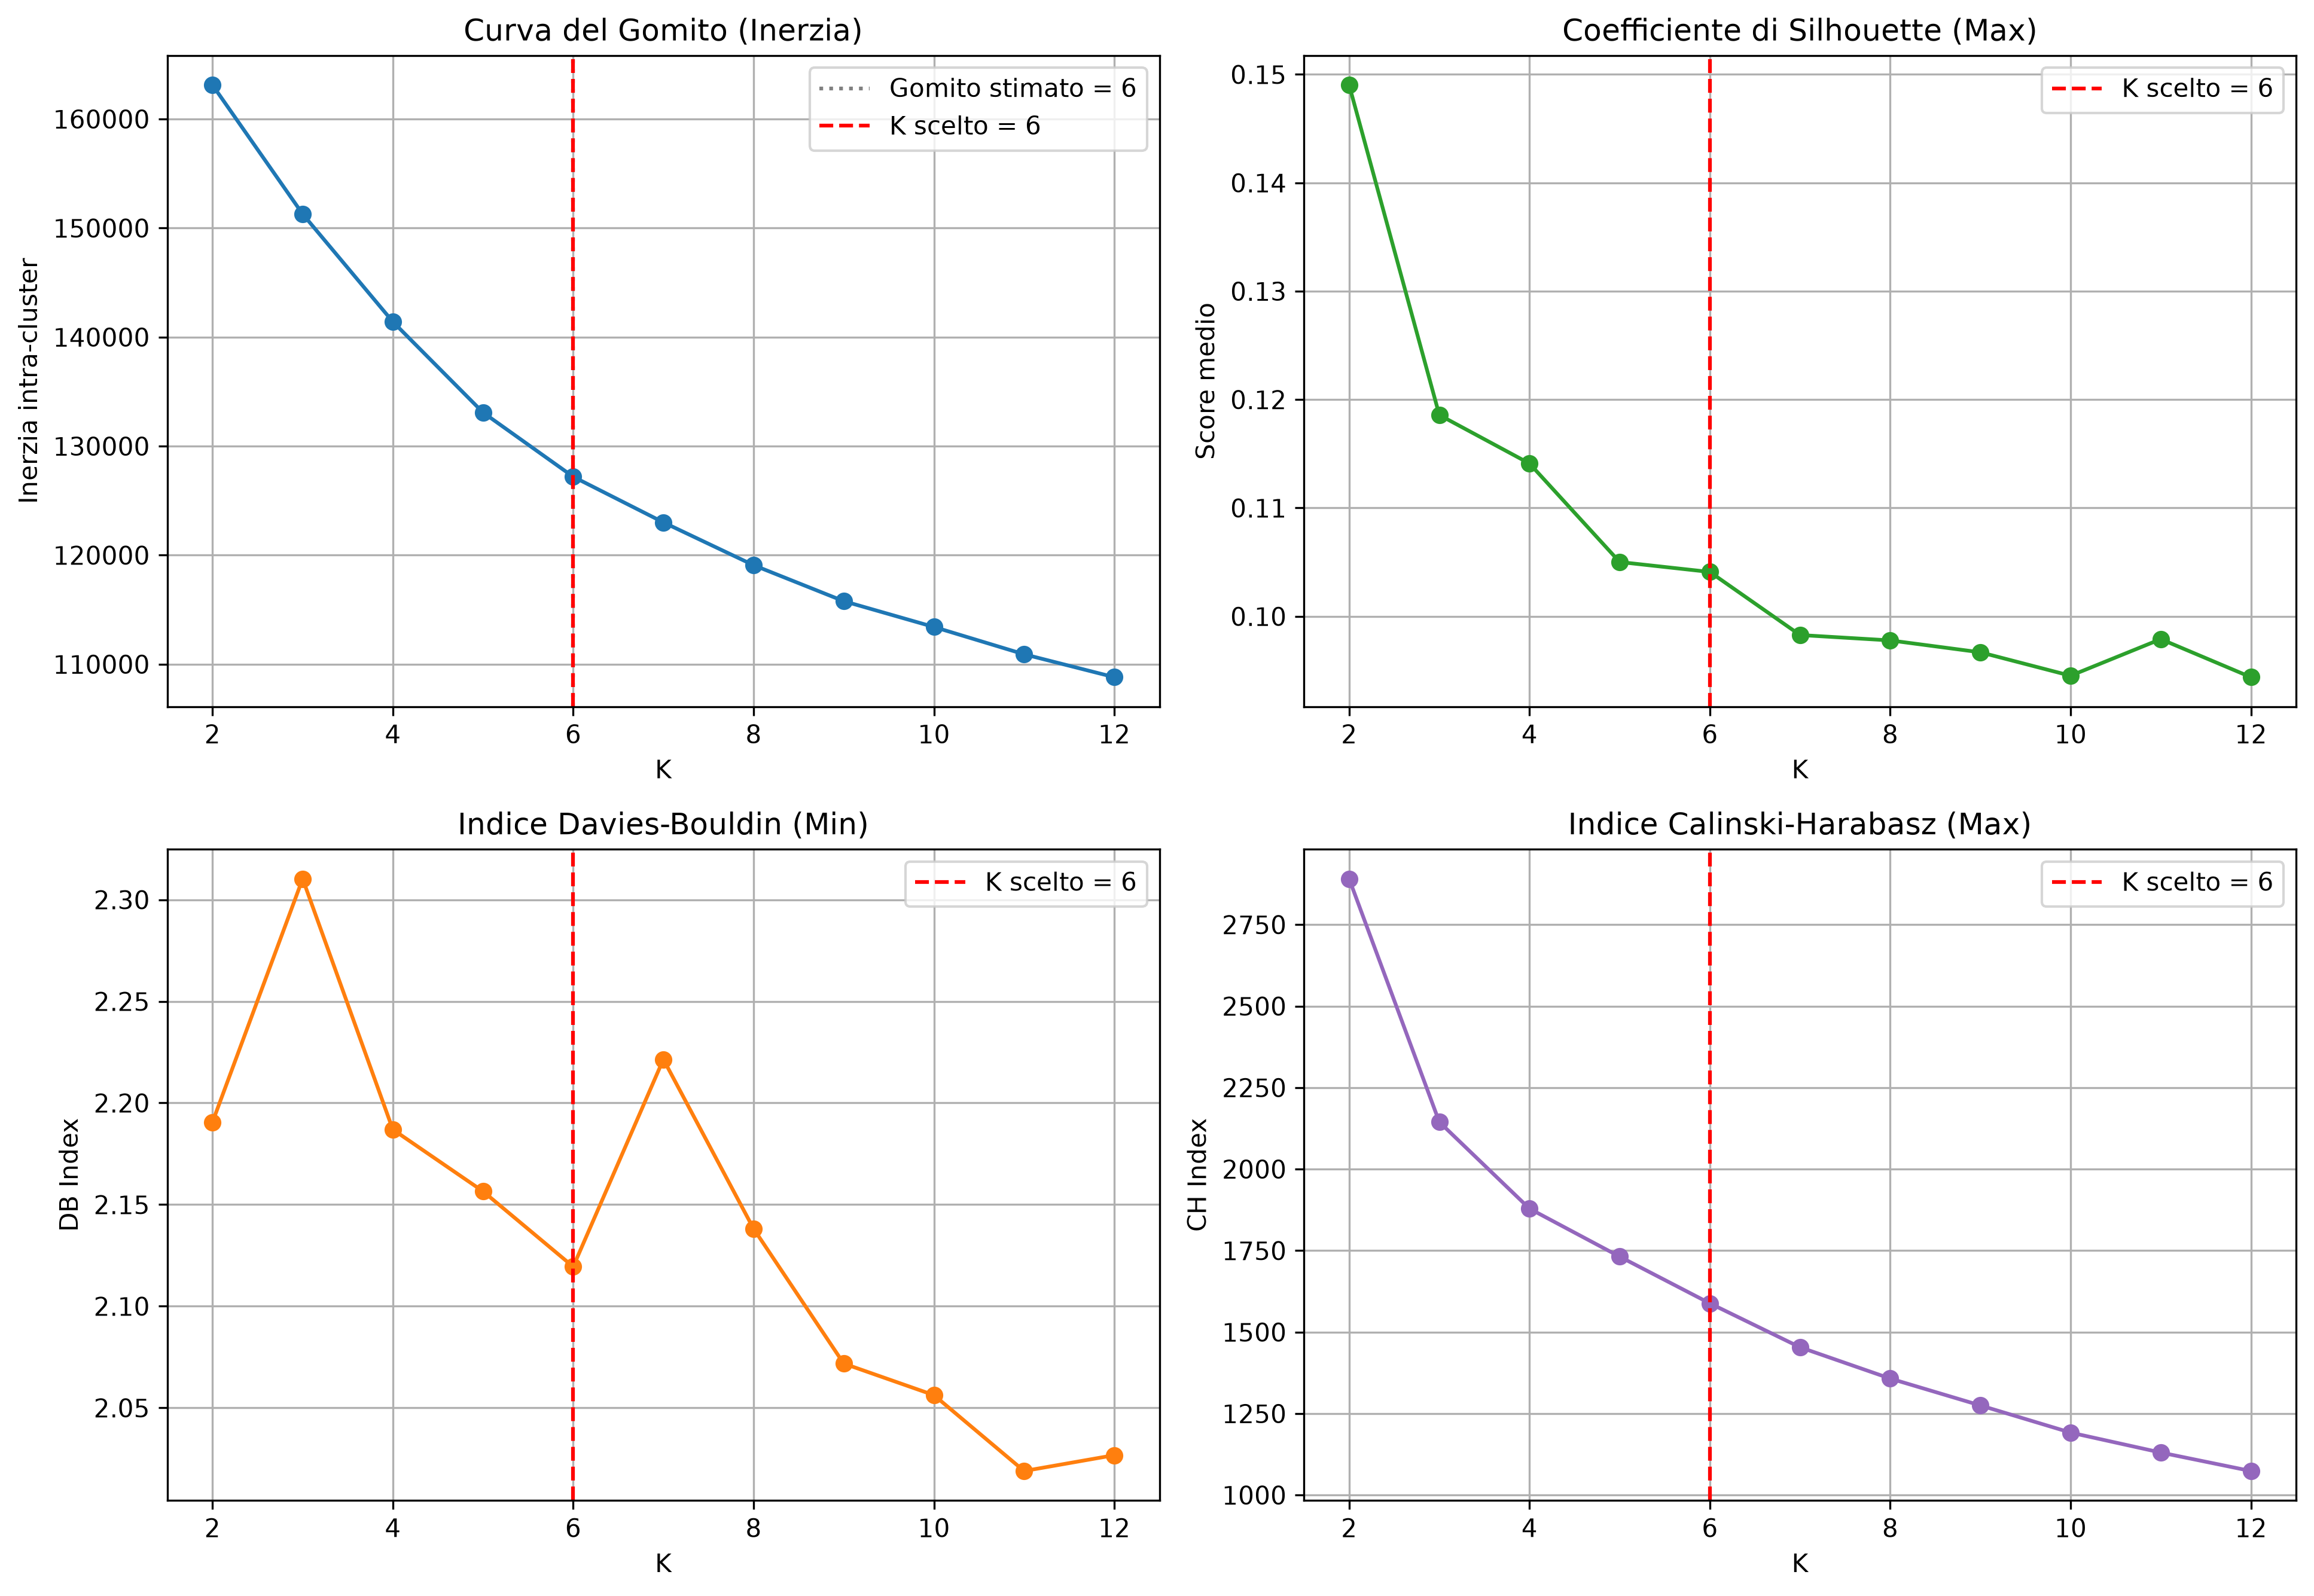
\includegraphics[width=\textwidth]{elbow_curve.png}
    \caption{Le quattro metriche per la selezione del $K$ ottimale:
    Curva del Gomito (Inerzia), Coefficiente di Silhouette,
    Indice di Davies-Bouldin e Indice di Calinski-Harabasz.
    La linea tratteggiata rossa indica $K=6$.}
    \label{fig:k_selection}
\end{figure}

\subsection{Visualizzazione Avanzata con Yellowbrick}

La libreria Yellowbrick ha fornito tre visualizzazioni diagnostiche
complementari che confermano la validità della partizione scelta:

\begin{enumerate}
    \item \textbf{KElbowVisualizer}: individuazione automatica del punto
    di gomito con indicatore visivo.

    \item \textbf{SilhouetteVisualizer}: profilo di silhouette per $K=6$,
    che mostra la densità e l'eventuale sbilanciamento dei cluster. Ogni
    ``lama'' del grafico rappresenta un cluster: la larghezza indica la
    dimensione, l'estensione orizzontale la coesione interna.

    \item \textbf{InterclusterDistance}: proiezione 2D dei centroidi con
    cerchi proporzionali alla dimensione dei cluster, per valutare la
    sovrapposizione spaziale.
\end{enumerate}

\begin{figure}[H]
    \centering
    
\includegraphics[width=0.65\textwidth]{silhouette_curve.png}
    \caption{Profilo Silhouette per $K=6$ (Yellowbrick). Ogni ``lama''
    rappresenta un cluster: la coesione interna è indicata dall'ampiezza
    orizzontale, la linea tratteggiata verticale segna la media globale.}
    \label{fig:yb_silhouette}
\end{figure}

\begin{figure}[H]
    \centering
    
\includegraphics[width=0.65\textwidth]{yb_intercluster.png}
    \caption{Mappa delle distanze inter-cluster (Yellowbrick). I centroidi
    sono proiettati in 2D; la dimensione dei cerchi è proporzionale al
    numero di pixel assegnati a ciascun cluster.}
    \label{fig:yb_intercluster}
\end{figure}

\subsection{Proiezione PCA dei Cluster}

La Figura~\ref{fig:pca} mostra la proiezione dei cluster nello spazio
delle prime due componenti principali. La separazione visiva dei cluster
conferma che le feature ingegnerizzate catturano strutture significative
nei dati, anche se la sovrapposizione parziale è attesa dato che la PCA
a due componenti comprime 13 dimensioni.

\begin{figure}[H]
    \centering
    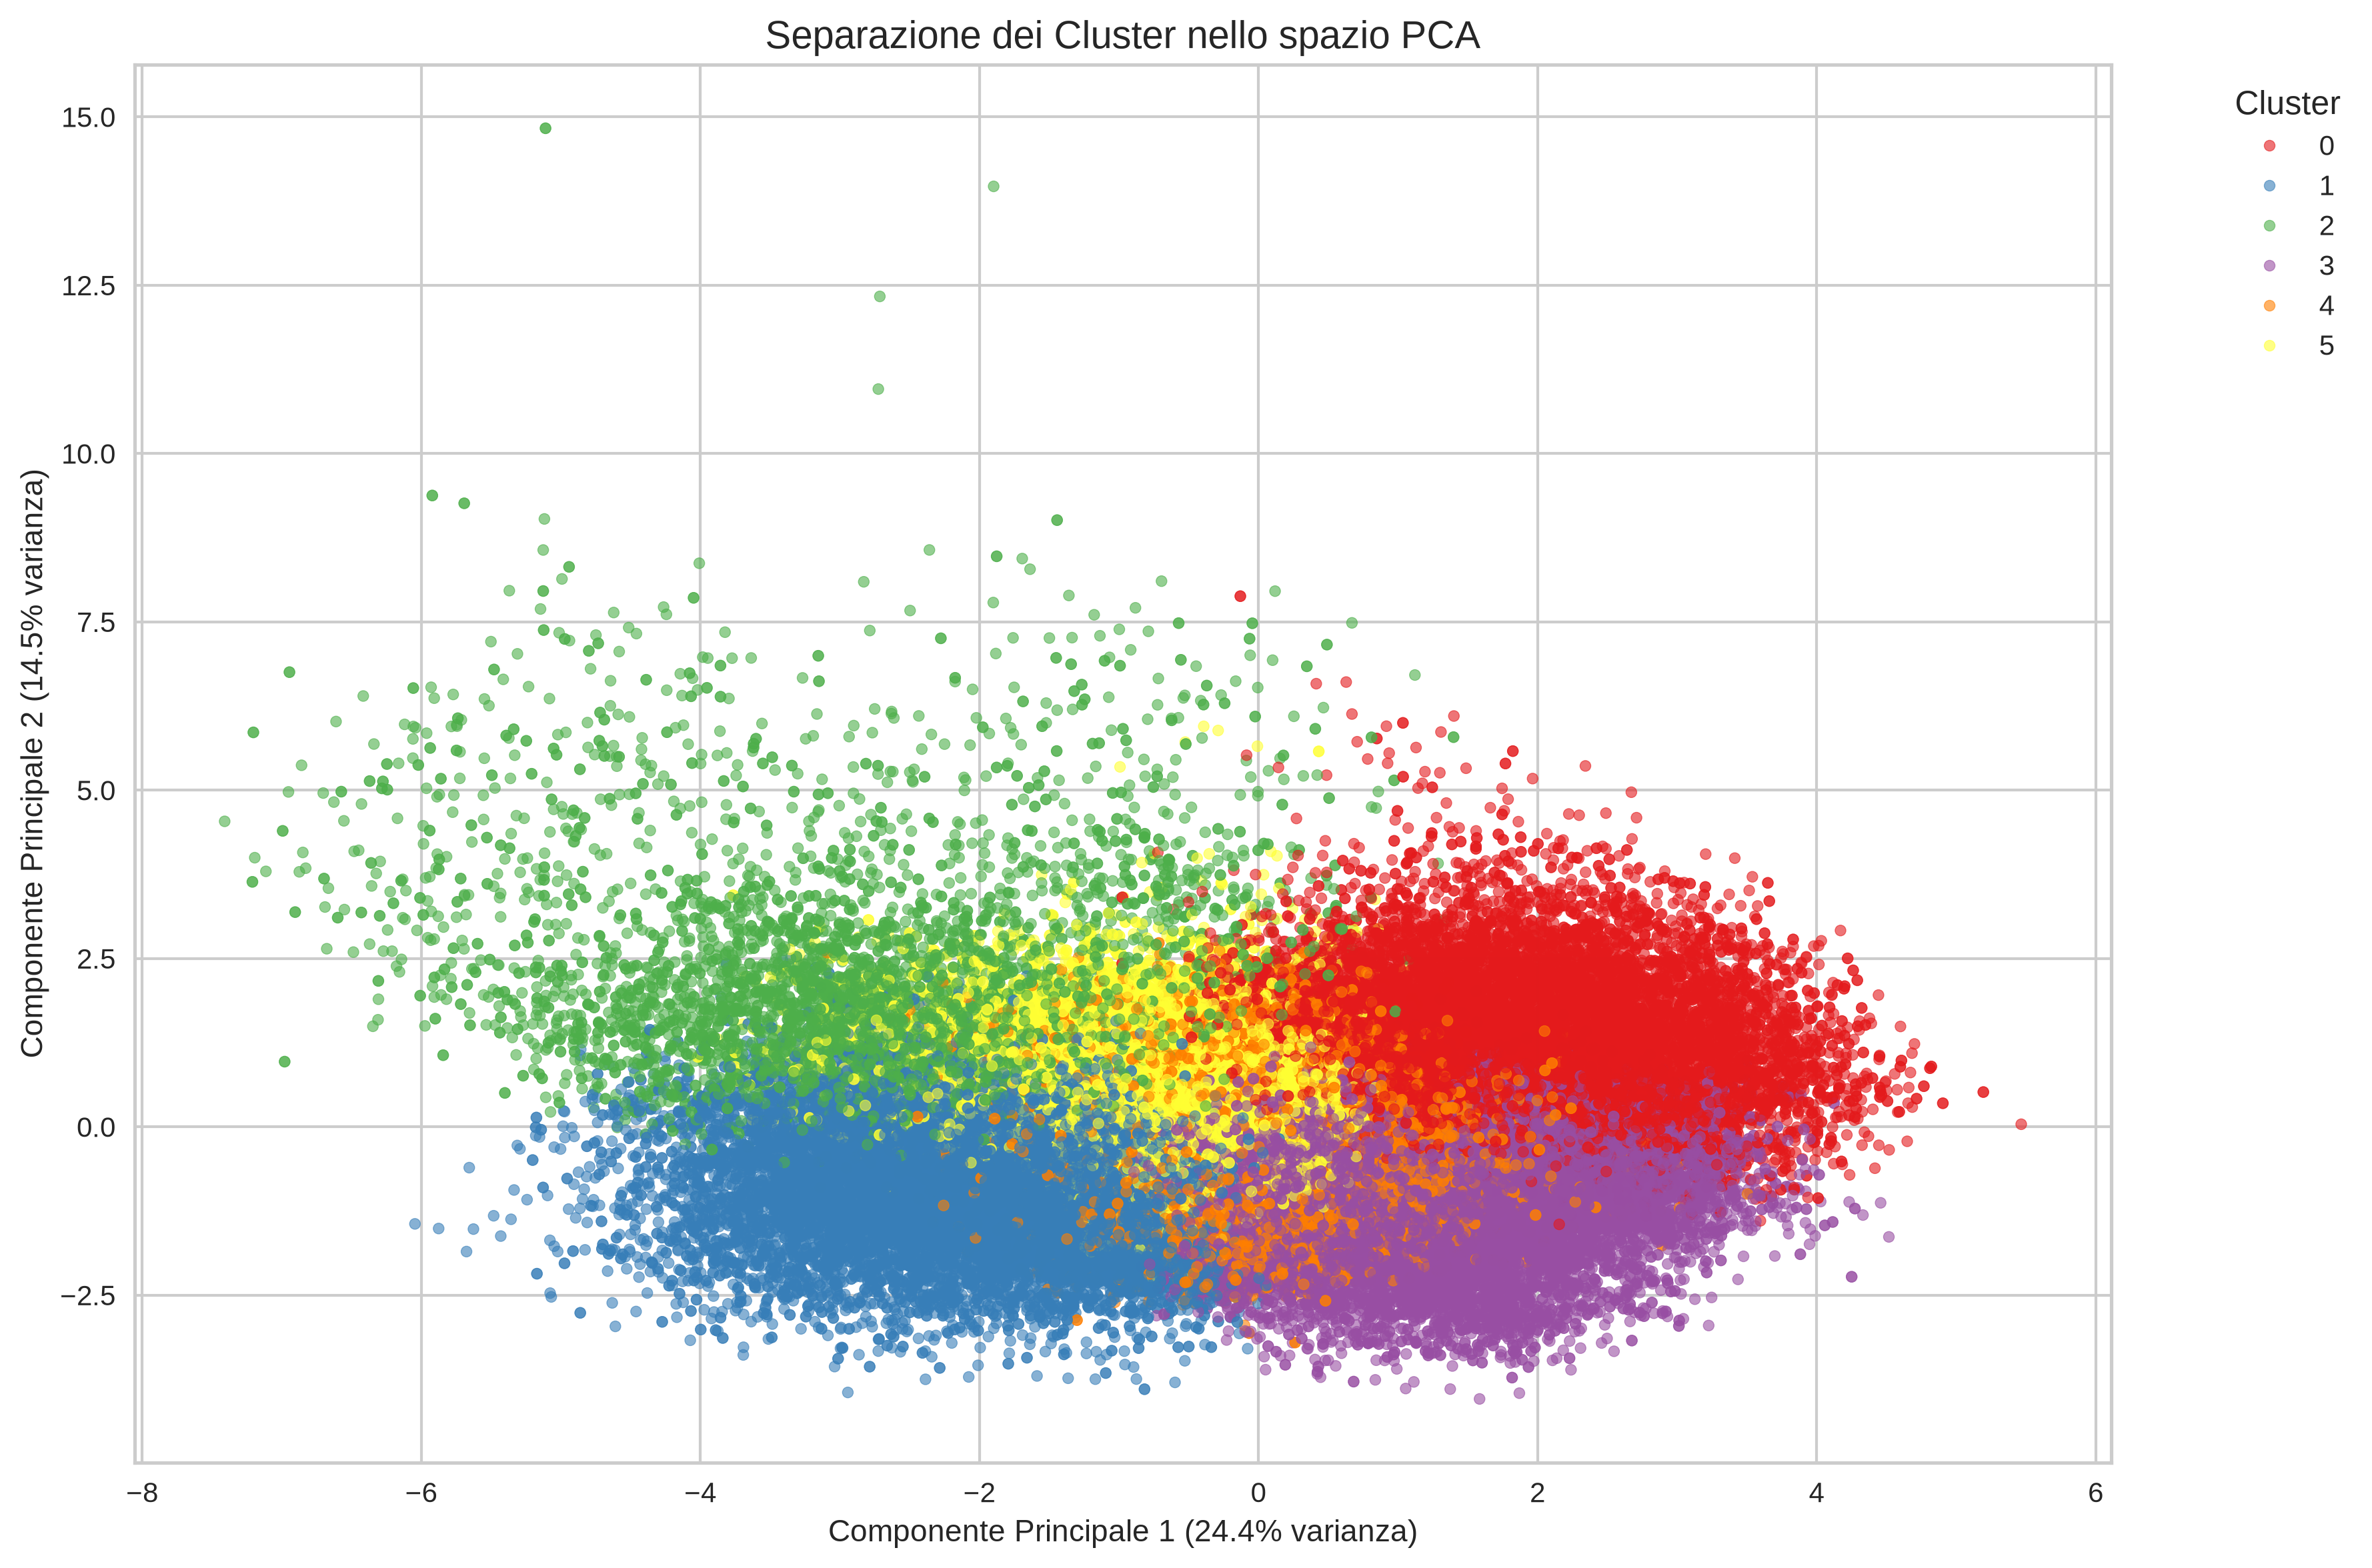
\includegraphics[width=0.75\textwidth]{pca_clusters.png}
    \caption{Proiezione PCA 2D dei cluster \kmeans{} con $K=6$. Le
    percentuali sugli assi indicano la varianza spiegata da ciascuna
    componente principale.}
    \label{fig:pca}

    
\end{figure}

L'ispezione dei coefficienti di correlazione (loadings) delle prime due componenti principali ne chiarisce il significato fisico: la prima componente (PC1, 24.4\% della varianza) è dominata lungo la direzione positiva dai gradienti di argilla (\texttt{clay\_grad}) e negativamente da quelli di sabbia (\texttt{sand\_grad}), separando chiaramente i suoli a evoluzione tessiturale fine da quelli più grossolani (a sinistra). La seconda componente (PC2, 14.5\% della varianza) è correlata prevalentemente alle variazioni di densità apparente (\texttt{bdod\_grad}) e di conducibilità idraulica, consentendo di distinguere verso l'alto i suoli a rapida compattazione sub-superficiale.

\subsection{Mappatura Spaziale dei Cluster}

Nonostante l'algoritmo non abbia ricevuto informazioni spaziali
(coordinate geografiche), i cluster assumono una distribuzione
geografica coerente con la geomorfologia della Capitanata
(Figure~\ref{fig:mappa_kmeans}--\ref{fig:mappe_alt}).

\begin{figure}[H]
    \centering
    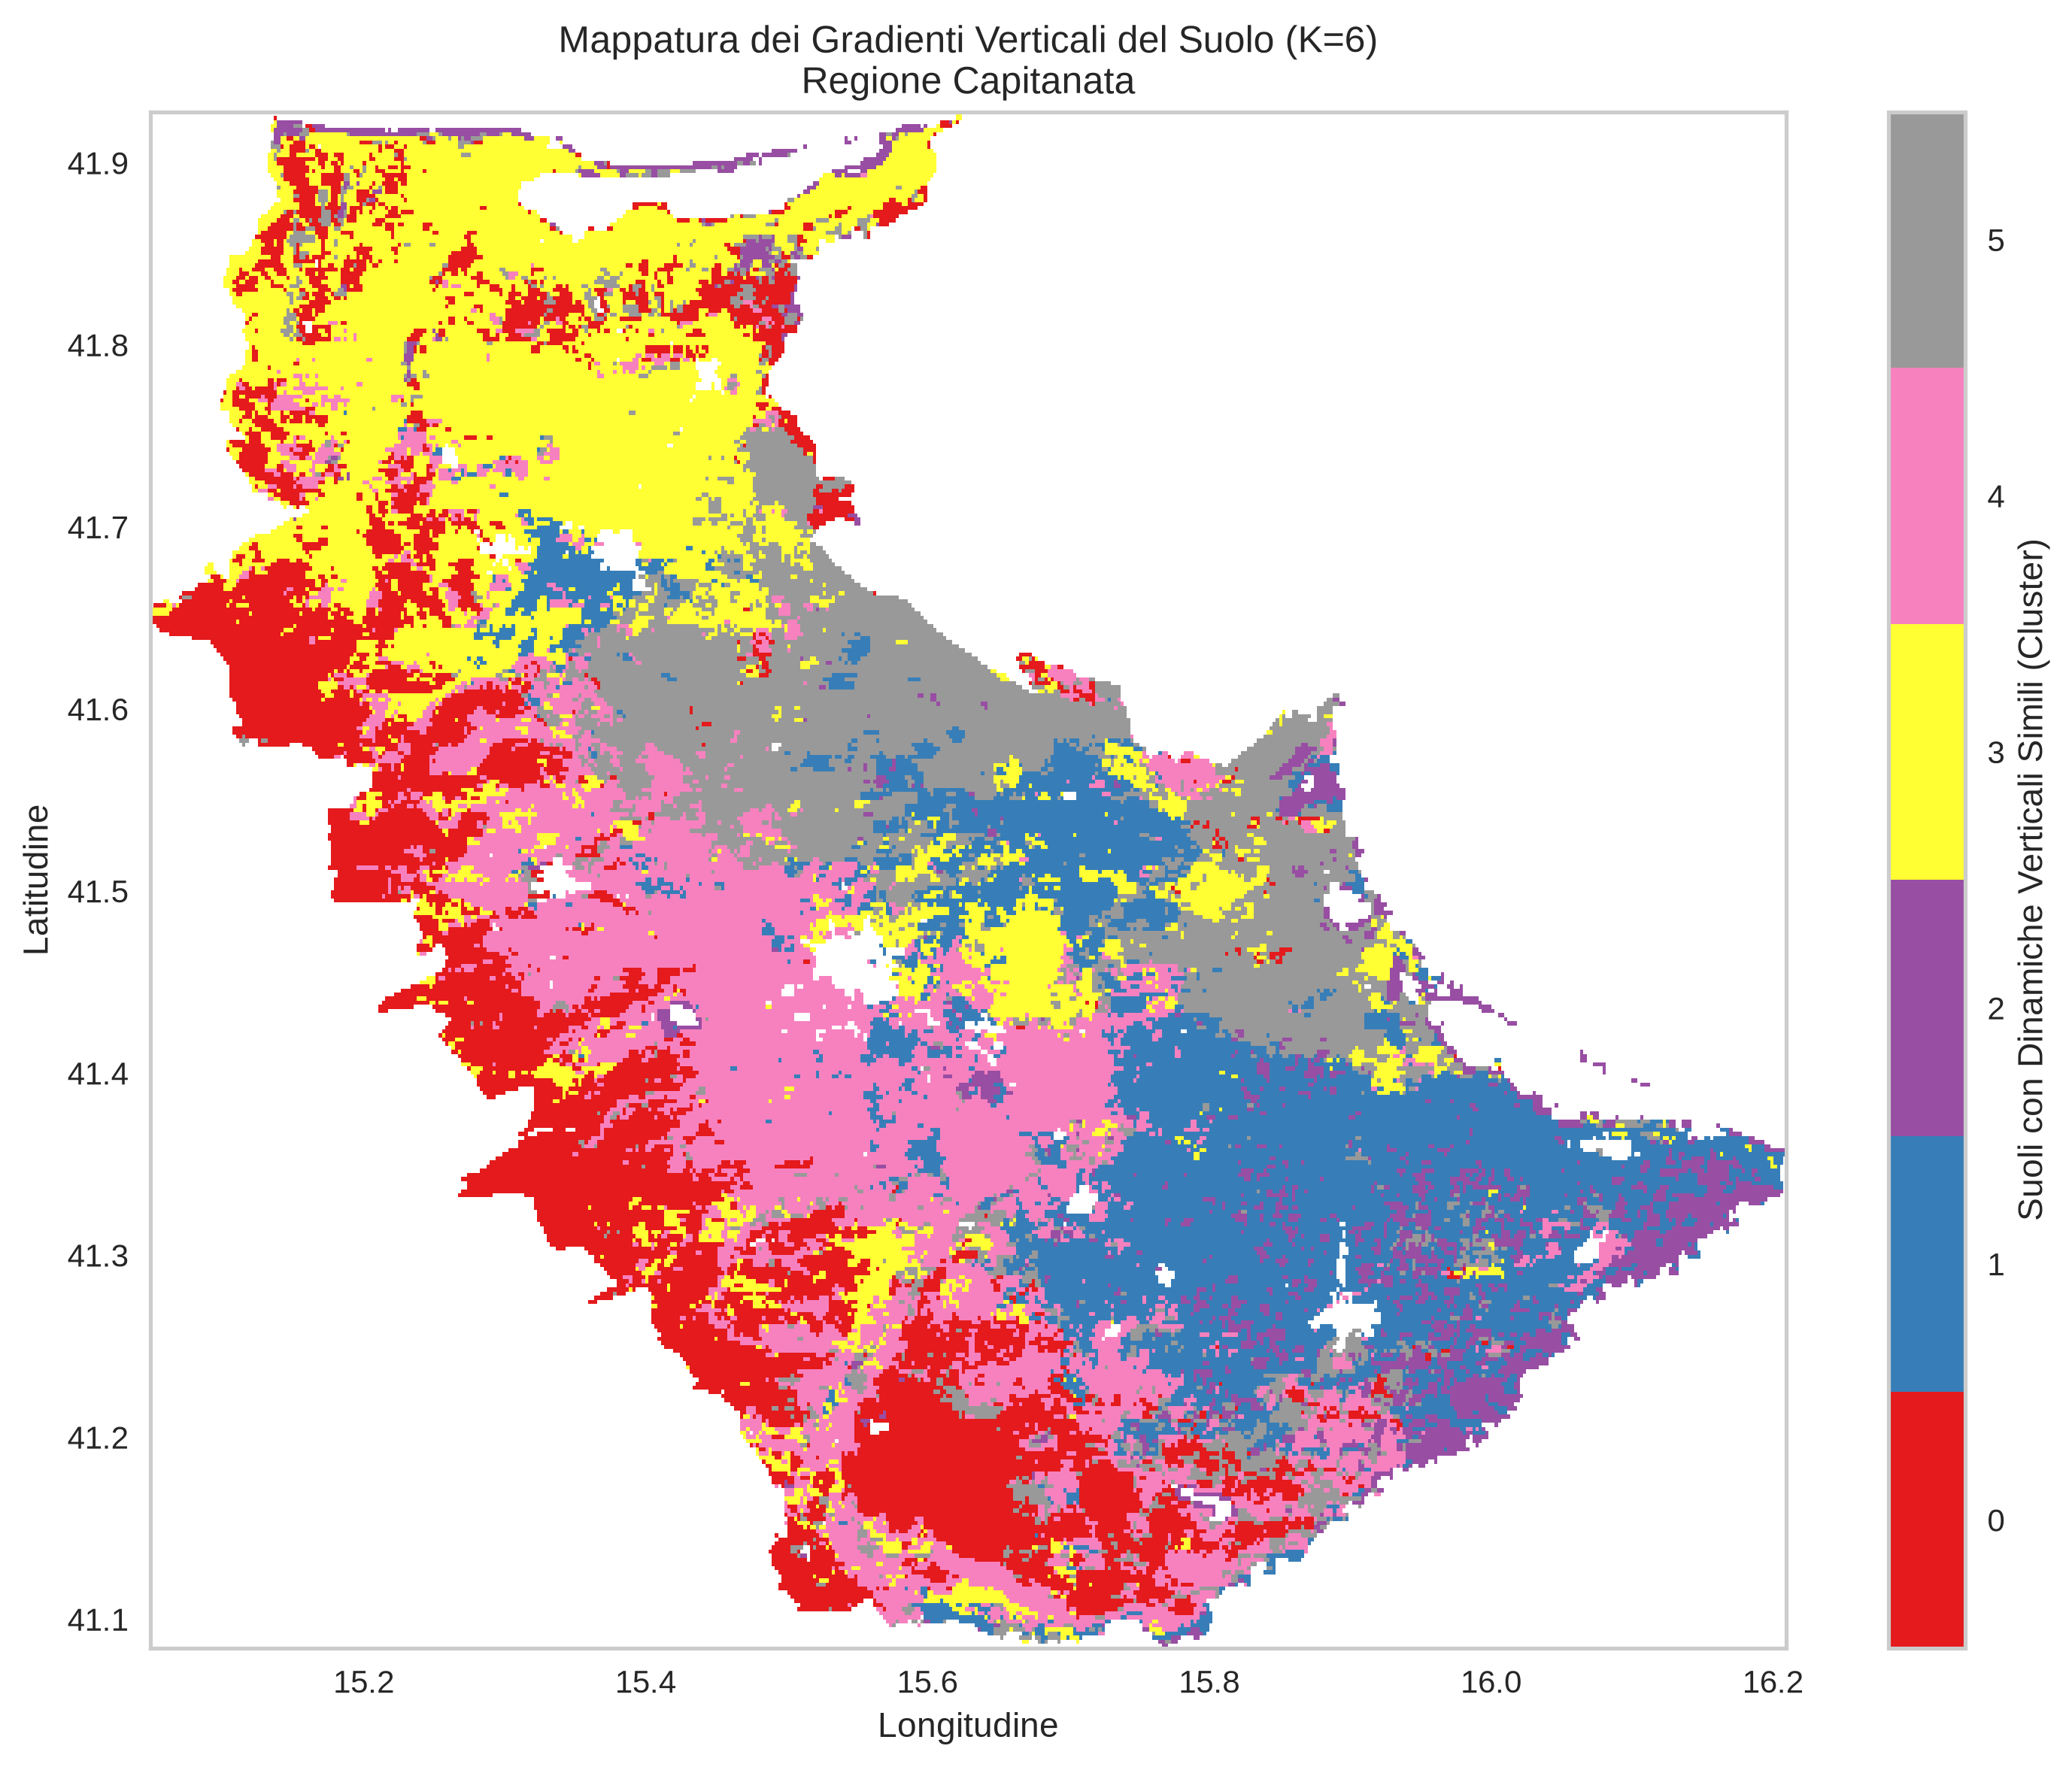
\includegraphics[width=0.8\textwidth]{mappa_kmeans.png}
    \caption{Mappatura spaziale dei cluster \kmeans{} con \kval{6}
    sulla regione Capitanata. La coerenza geografica dei cluster
    conferma la validità pedologica dell'analisi.}
    \label{fig:mappa_kmeans}
\end{figure}

\begin{figure}[H]
    \centering
    \begin{subfigure}[b]{0.48\textwidth}
        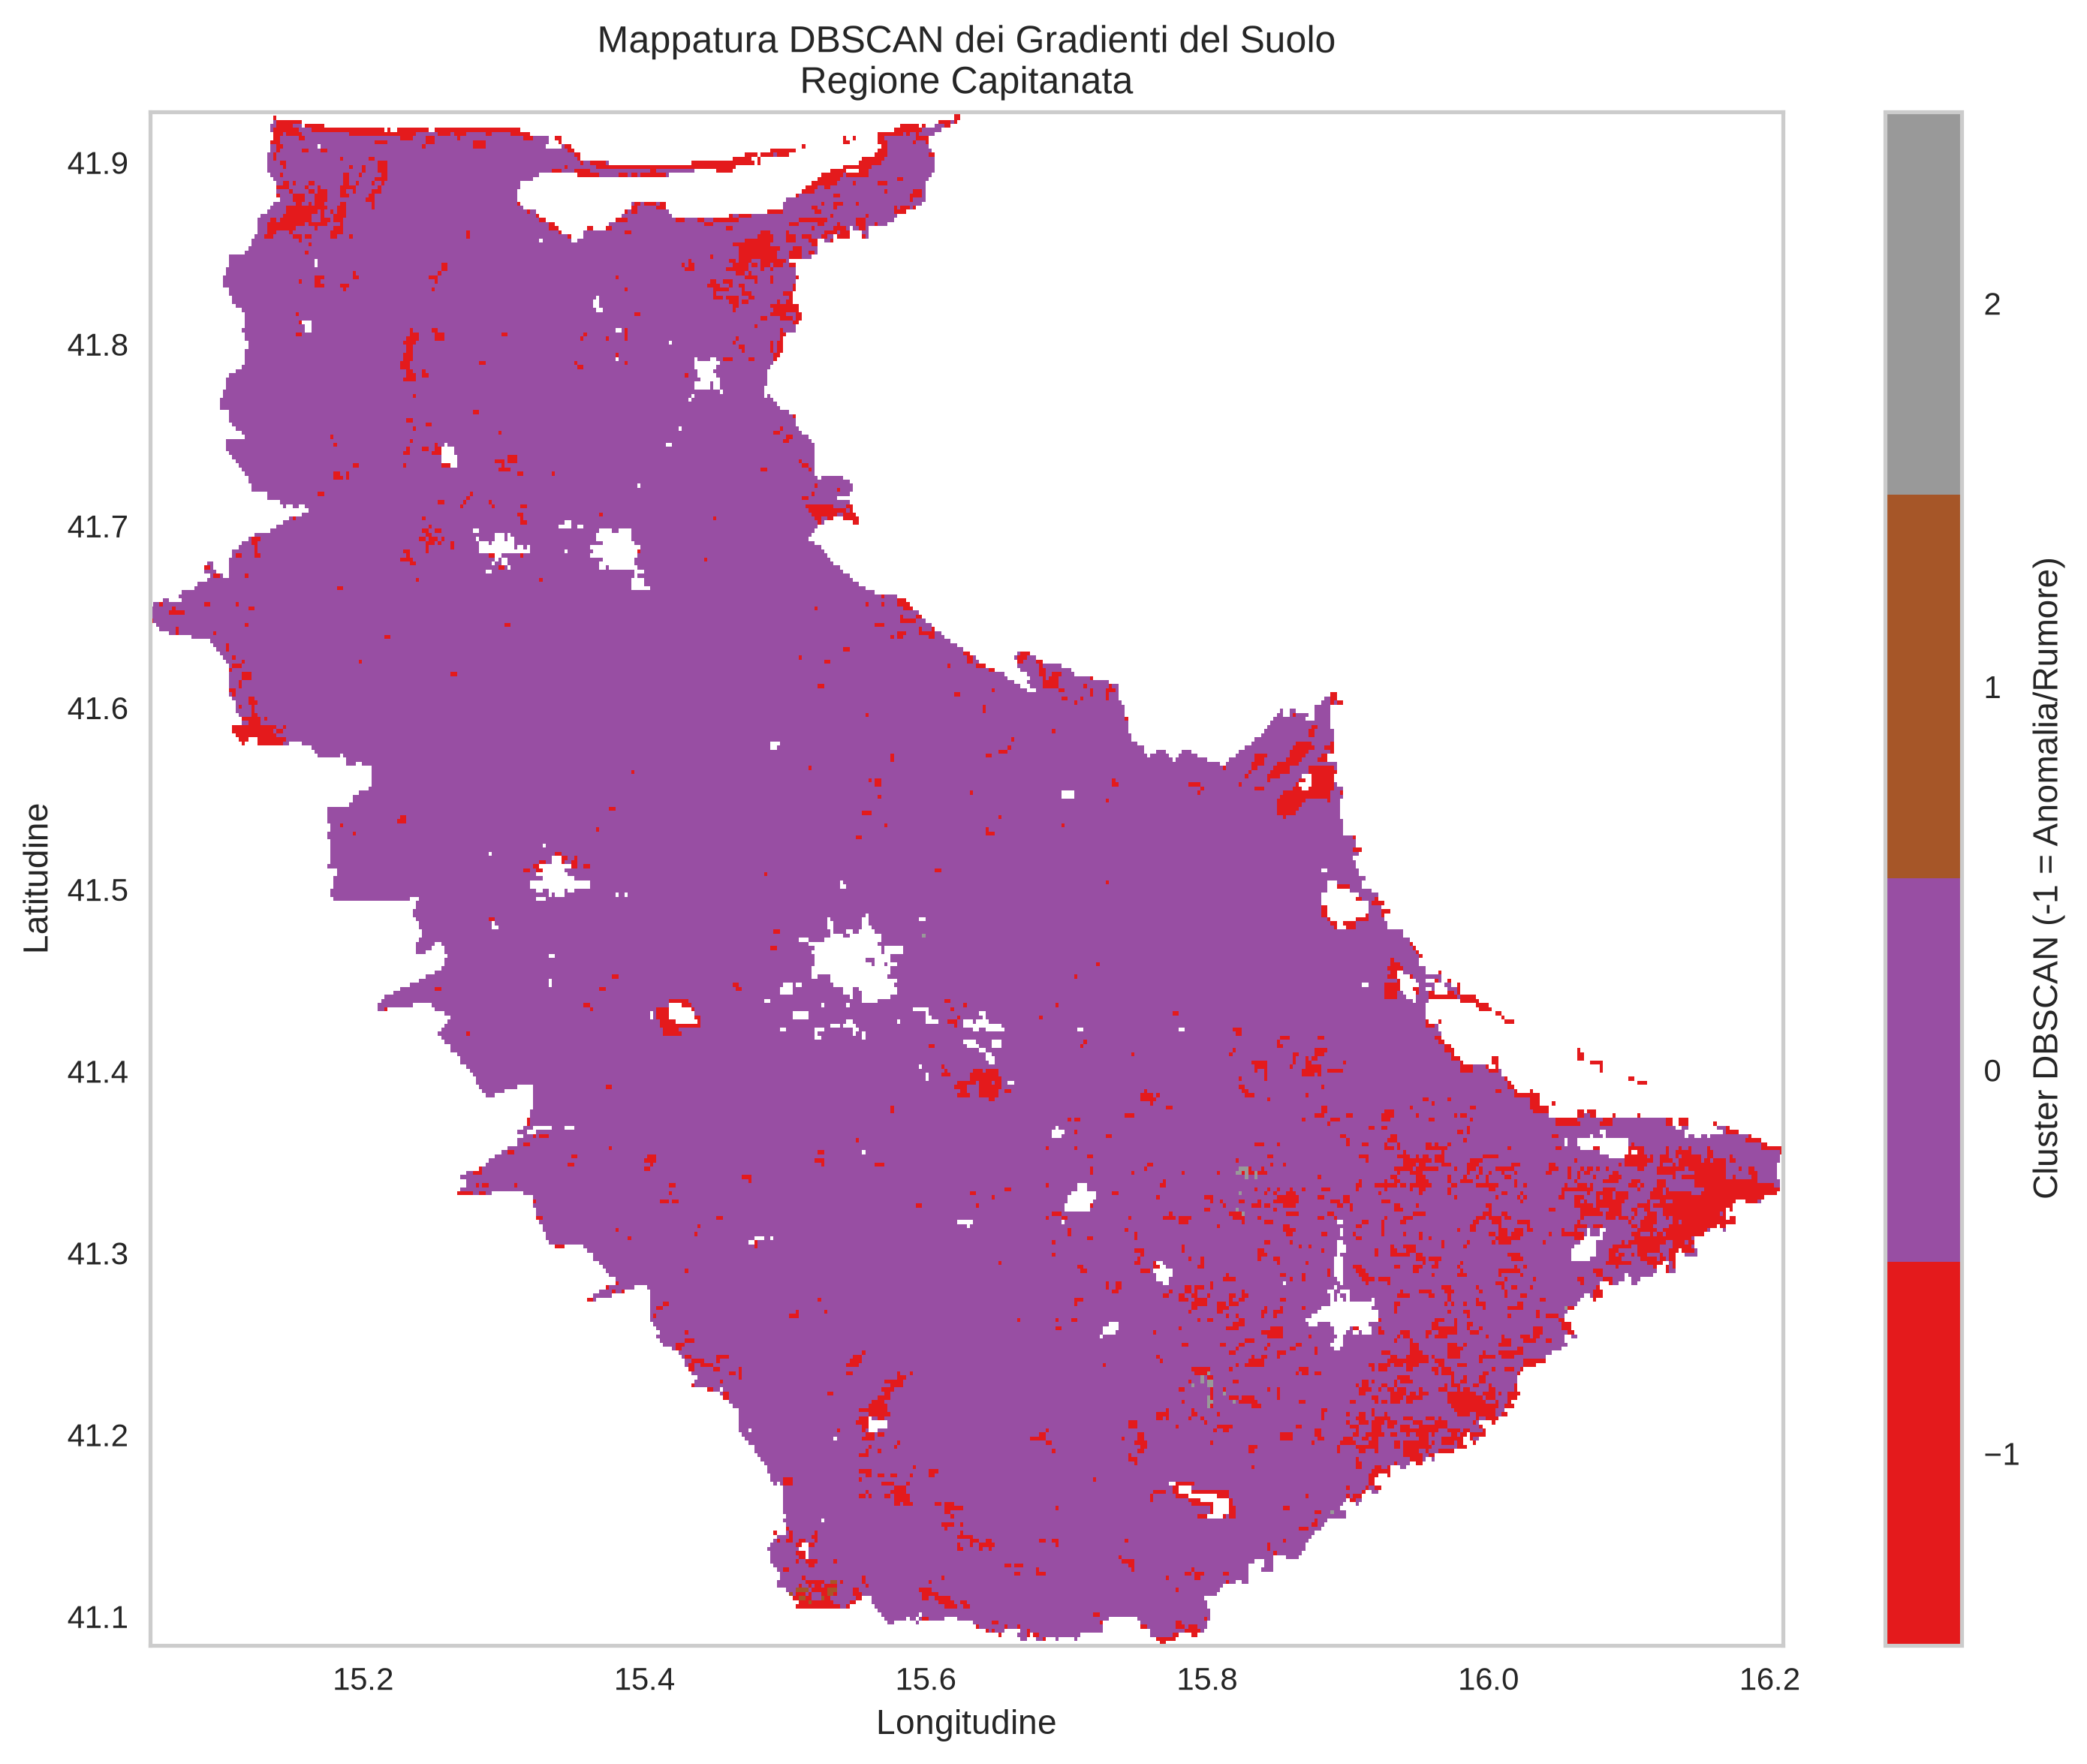
\includegraphics[width=\textwidth]{mappa_dbscan.png}

        \caption{DBSCAN ($\varepsilon=1.9$, \texttt{min\_samples}=26).}
        \label{fig:mappa_dbscan}
    \end{subfigure}
    \hfill
    \begin{subfigure}[b]{0.48\textwidth}
        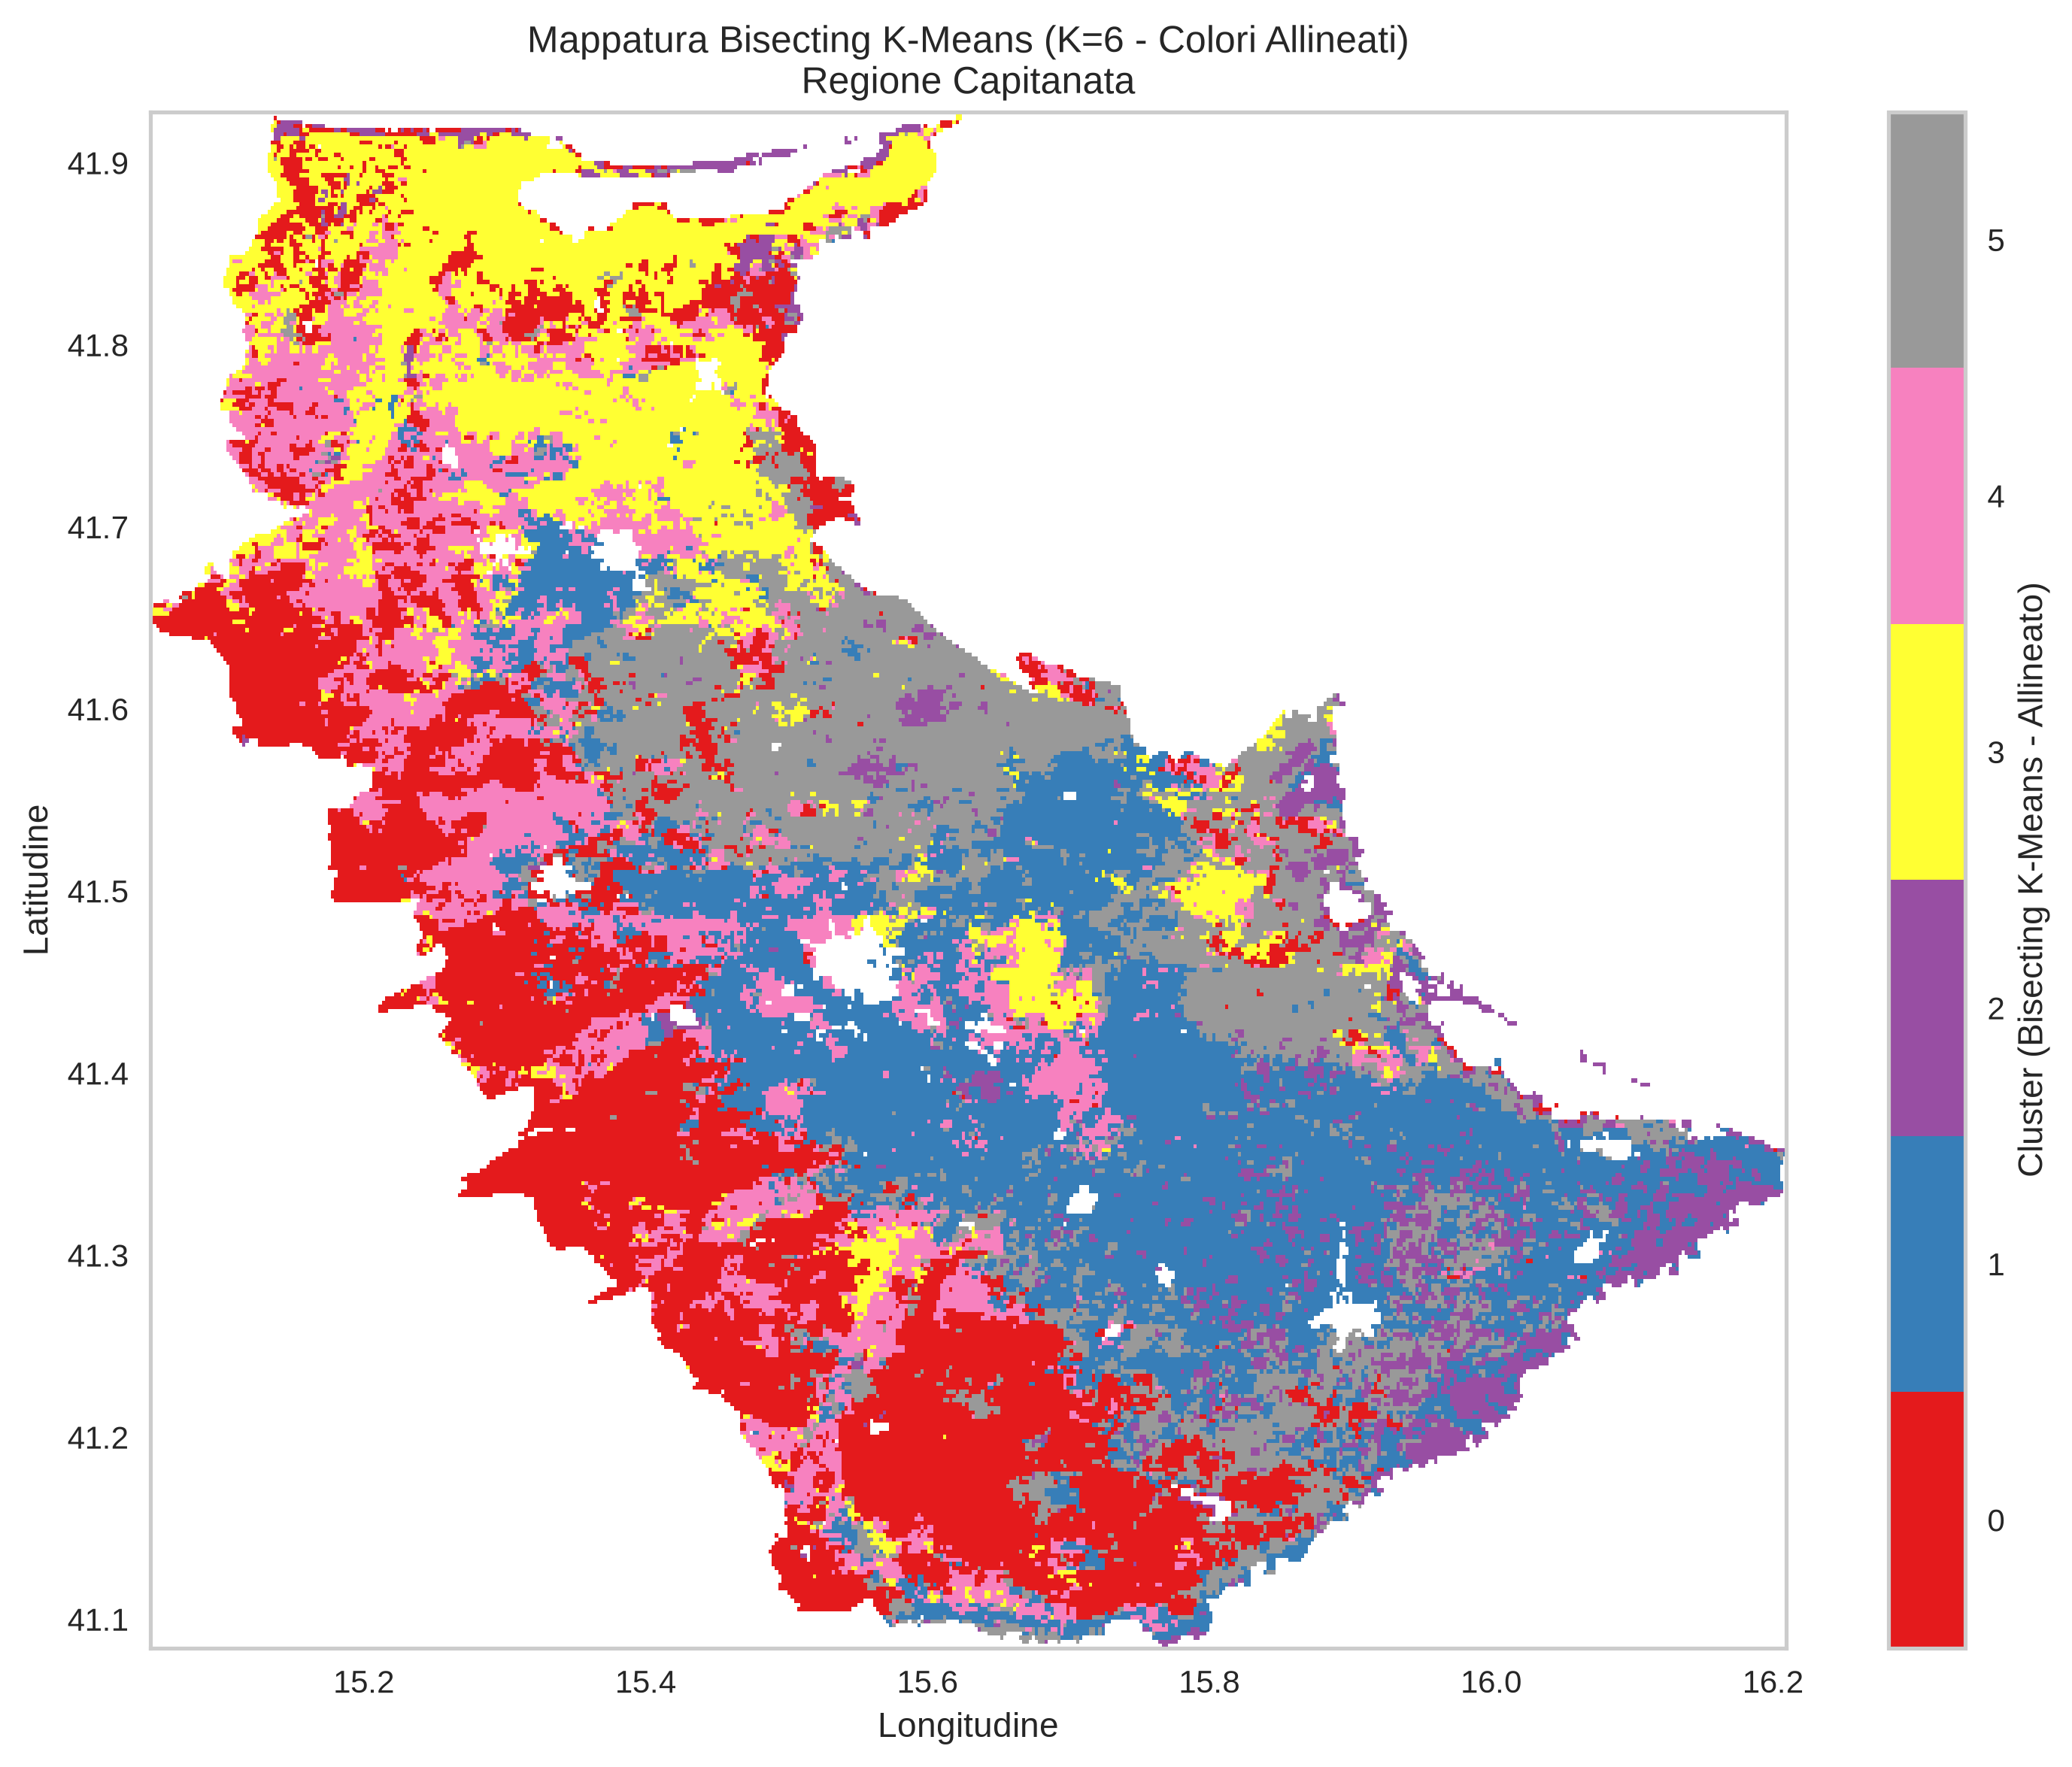
\includegraphics[width=\textwidth]{mappa_bisecting.png}

        \caption{Bisecting \kmeans{} ($K=6$).}
        \label{fig:mappa_bisecting}
    \end{subfigure}
    \caption{Confronto delle mappature spaziali per DBSCAN e Bisecting
    \kmeans{}.}
    \label{fig:mappe_alt}
\end{figure}

\paragraph{Analisi Critica del Fallimento di DBSCAN.}
Sebbene l'euristica della curva $k$-NN avesse suggerito la combinazione parametrica $\epsilon = 2.6$ e $\text{min\_samples} = 26$, i risultati sperimentali (ottenuti con $\epsilon = 1.9$) mostrano un sostanziale collasso dell'algoritmo su un unico macro-cluster dominante, con il $6.20\%$ dei pixel marginali classificati come rumore. Le motivazioni teoriche e pratiche di tale comportamento sono principalmente due:

\begin{enumerate}
    \item \textbf{Continuità del continuum pedologico:} Il paradigma di DBSCAN presuppone regioni ad alta densità separate da ampie zone a densità prossima allo zero (vuoti dimensionali). Le variabili pedologiche e i rispettivi gradienti verticali, al contrario, variano nello spazio geografico e geometrico in maniera intrinsecamente continua e graduale. La densità dei punti nello spazio delle feature non presenta separazioni nette, bensì una transizione continua di densità che innesca una reazione a catena per densità-raggiungibilità (\emph{density-reachability}), agglomerando quasi la totalità dei dati in un'unica componente connessa.
    
    \item \textbf{Maledizione della dimensionalità (\emph{Curse of Dimensionality}):} Nello spazio $13$-dimensionale dei gradienti standardizzati, il contrasto tra la distanza dal vicino più prossimo e la distanza dal punto più lontano tende a ridursi notevolmente (\emph{distance concentration phenomenon}). In tale contesto iper-dimensionale, il concetto di raggio di vicinato globale ($\epsilon$) perde efficacia: un incremento infinitesimo di $\epsilon$ induce la fusione improvvisa di cluster contigui, mentre una minima diminuzione classifica arbitrariamente gran parte del dataset come rumore, rendendo insoddisfacente la separazione basata su densità stazionaria globale.
\end{enumerate}
Per tale motivo, gli approcci partizionali (K-Means) e probabilistici (GMM), operando mediante centri di aggregazione o funzioni di covarianza ellissoidali, risultano matematicamente e fisicamente più idonei per la discretizzazione di distribuzioni unimodali e continue tipiche delle scienze della Terra.

\subsection{Profilazione dei Cluster (Risultati di K-Means)}

La heatmap dei centroidi standardizzati (Z-score) permette di
interpretare il ``profilo agronomico'' di ciascun cluster
(Figura~\ref{fig:profili}). Valori fortemente positivi (rossi) indicano
che il gradiente di una determinata variabile è nettamente superiore
alla media regionale; valori negativi (blu) indicano il comportamento
opposto. Questa rappresentazione consente di associare a ciascun cluster
una descrizione pedologica qualitativa.

\begin{figure}[H]
    \centering
    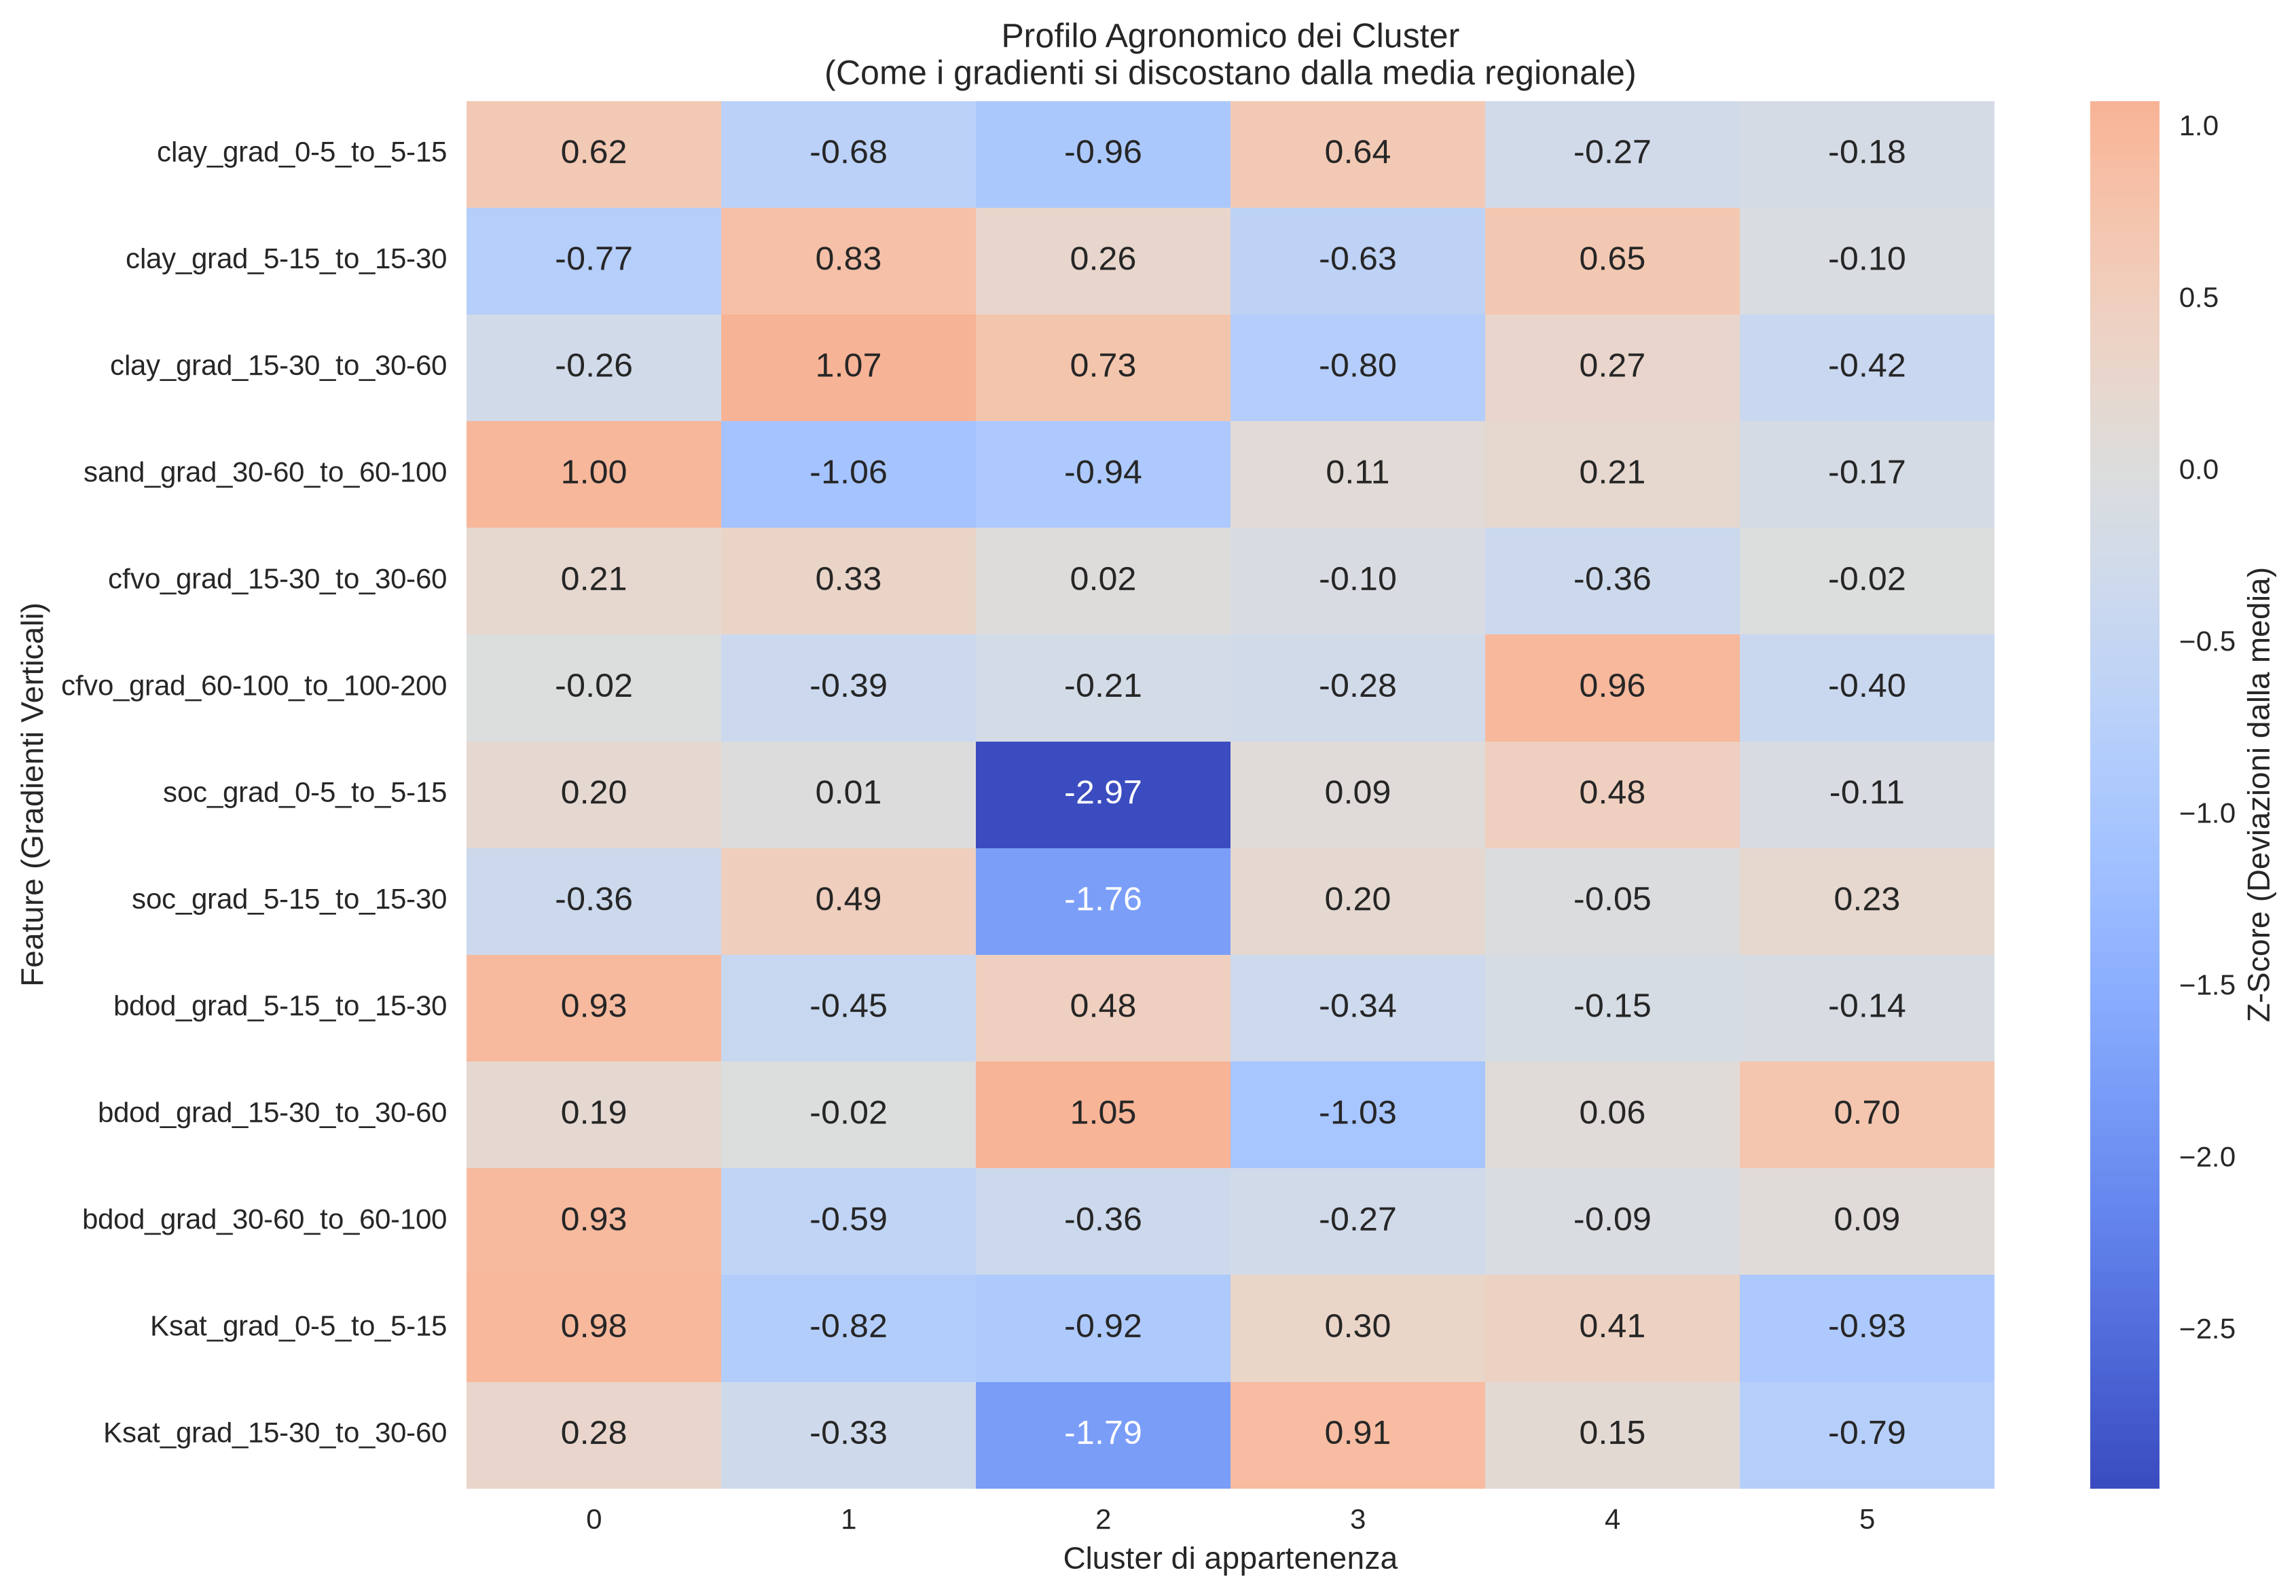
\includegraphics[width=0.85\textwidth]{profili_cluster.png}
    \caption{Profilo agronomico dei 6 cluster basato sugli Z-score dei
    centroidi. Valori positivi (rossi) indicano gradienti superiori alla
    media regionale; valori negativi (blu) indicano gradienti inferiori.}
    \label{fig:profili}
\end{figure}

Dall'analisi congiunta degli $Z$-score dei centroidi e della distribuzione spaziale sul territorio, emergono sei profili pedologici ben differenziati:

\begin{itemize}
    \item \textbf{Cluster 0 -- Dinamiche superficiali e compattazione profonda (Rosso):} 
    Caratterizzato da marcati gradienti positivi superficiali di argilla ($+0.62$) e conduttività idraulica $K_{\text{sat}}$ ($+0.98$), accompagnati da un sensibile incremento della densità apparente negli orizzonti profondi (\texttt{bdod\_grad\_30-60\_to\_60-100} pari a $+0.93$). Spazialmente si concentra lungo la fascia sub-appenninica e pedemontana, riflettendo suoli con netto passaggio a substrati più compatti.

    \item \textbf{Cluster 1 -- Lisciviazione argillosa e sviluppo dell'orizzonte $B_t$ (Blu):} 
    Presenta il massimo accumulo verticale di argilla a profondità intermedie \\(\texttt{clay\_grad\_15-30\_to\_30-60} pari a $+1.07$) a fronte di un forte calo del gradiente di sabbia ($-1.06$). Identifica i suoli alluvionali di pianura soggetti a traslocazione e illuviazione di argilla (formazione di orizzonti diagnostici argillici $B_t$).

    \item \textbf{Cluster 2 -- Rapida de-sostanziazione e suola di lavorazione (Viola):} 
    È contraddistinto dall'anomalia negativa più estrema del dataset sul gradiente di carbonio organico (\texttt{soc\_grad\_0-5\_to\_5-15} a $-2.97$), associata a un forte gradiente positivo di densità apparente tra i 15 e i 60~cm ($+1.05$). Individua suoli intensamente coltivati soggetti a progressivo degrado organico superficiale e compattazione meccanica sub-superficiale (suola di aratura).

    \item \textbf{Cluster 3 -- Orizzonti permeabili a lenta variazione di densità (Giallo):} 
    Evidenzia un incremento del gradiente di $K_{\text{sat}}$ profonda ($+0.91$) e moderati gradienti argillosi superficiali ($+0.64$), con una densità apparente in netta controtendenza (\texttt{bdod\_grad\_15-30\_to\_30-60} pari a $-1.03$). Localizzato principalmente nel settore settentrionale della pianura, descrive suoli franchi a buona permeabilità strutturale.

    \item \textbf{Cluster 4 -- Contatto litologico e accumulo di scheletro profondo (Rosa):} 
    Rappresenta l'unico gruppo dominato da un marcato gradiente positivo di frammenti grossolani nello strato più profondo (\texttt{cfvo\_grad\_60-100\_to\_100-200} pari a $+0.96$), preservando al contempo un gradiente organico superficiale moderato ($+0.48$). Risulta coerente con le aree di transizione verso rilievi carsici o substrati rocciosi affioranti.

    \item \textbf{Cluster 5 -- Profili verticalmente omogenei a drenaggio ridotto (Grigio):} 
    Mostra gradienti prossimi allo zero o debolmente negativi su quasi tutte le frazioni granulometriche, accompagnati da una riduzione di conducibilità idraulica profonda ($-0.79$) e scheletro ($-0.40$). Rappresenta profili sedimentari stabili, scarsamente differenziati lungo i primi due metri di profondità.
\end{itemize}

\subsection{Risultati del GMM (Expectation-Maximization)}


\subsubsection{Selezione del Modello: BIC e AIC}
La Figura~\ref{fig:bic_aic} illustra l'andamento del Bayesian Information Criterion (BIC) e dell'Akaike Information Criterion (AIC) al variare del numero di componenti gaussiane ($K \in [2, 12]$). 

Entrambi i criteri mostrano una decrescita continua all'aumentare di $K$, comportamento tipico nei dataset geospaziali ad elevata numerosità campionaria dove l'aumento dei parametri liberi continua a incrementare marginalmente la log-verosimiglianza complessiva. Tuttavia, si osserva un chiaro cambio di pendenza con progressiva saturazione del gradiente di discesa attorno a $K=6$. 

Poiché l'obiettivo primario è il confronto strutturale controllato tra paradigmi di clustering differenti (partizionale, gerarchico, probabilistico), si è optato per fissare $K=6$. Tale scelta garantisce parsimonia parametrica, previene l'eccessiva frammentazione agronomica e consente un confronto diretto e consistente delle partizioni territoriali a parità di cardinalità dei gruppi.

\begin{figure}[H]
    \centering
    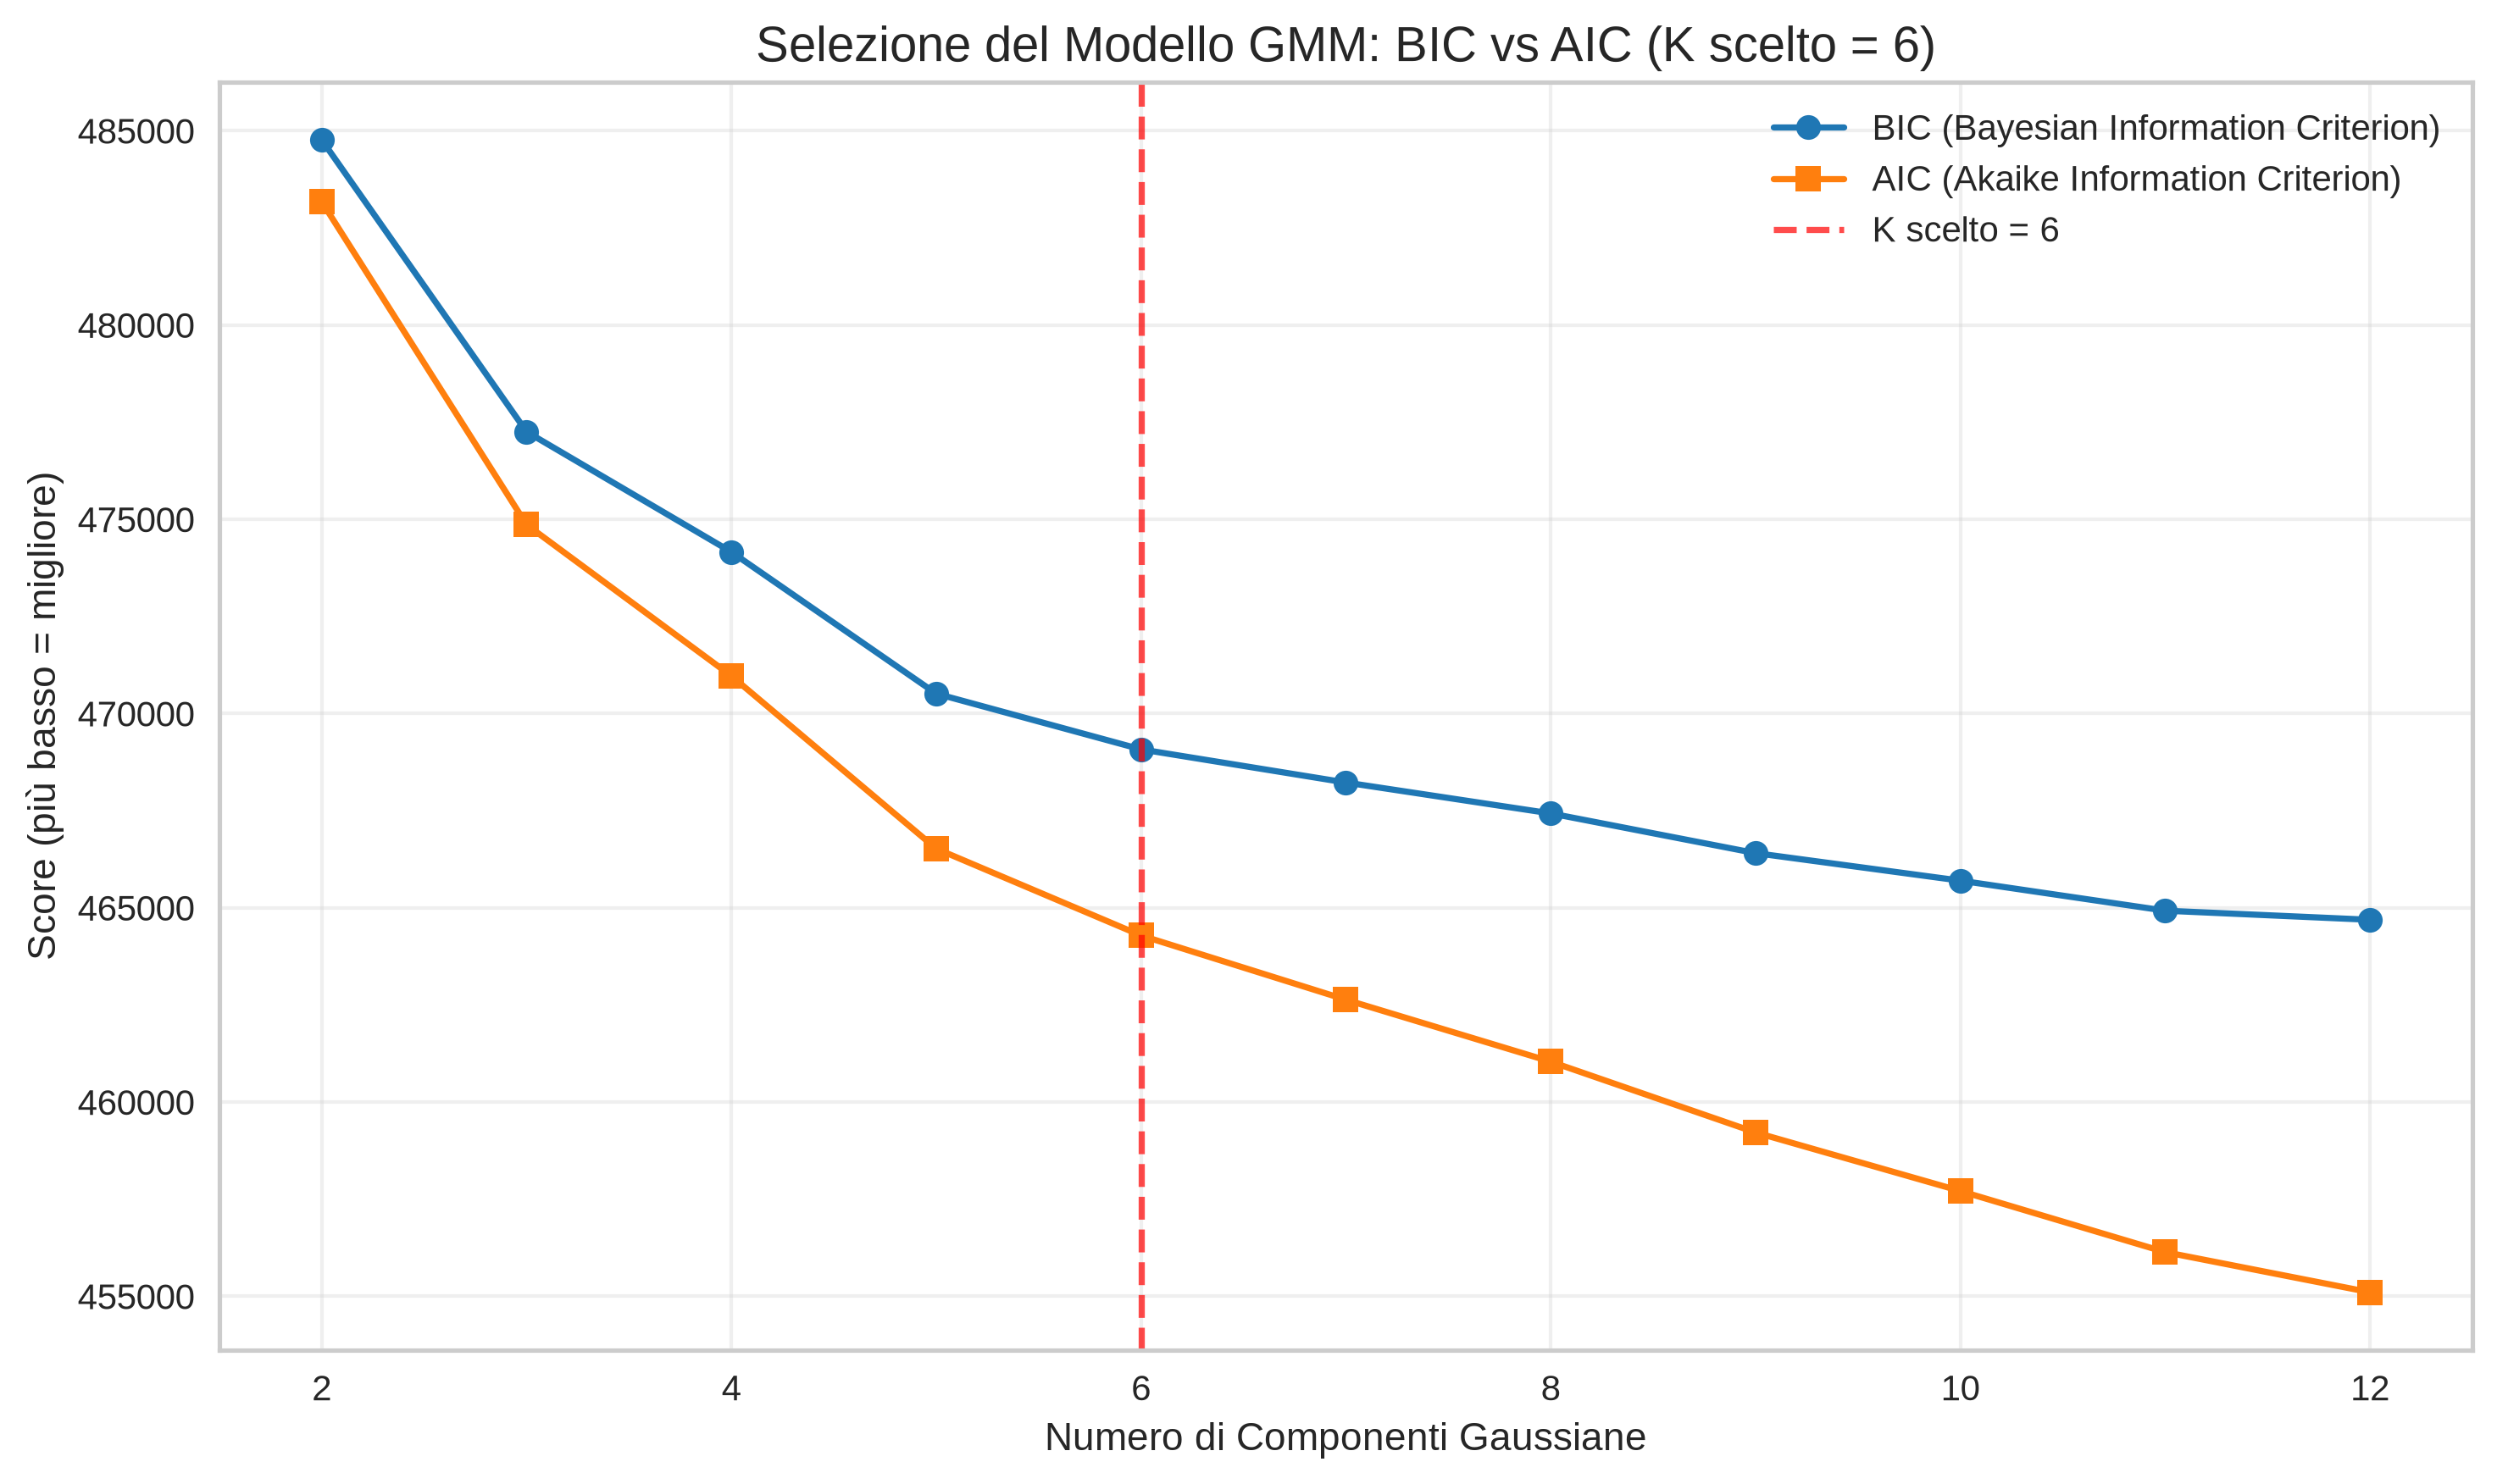
\includegraphics[width=0.7\textwidth]{bic_aic_gmm.png}
    \caption{Curve BIC e AIC per il GMM al variare del numero di
    componenti. La linea tratteggiata rossa indica $K=6$.}
    \label{fig:bic_aic}
\end{figure}

\subsubsection{Mappatura Spaziale GMM}

La Figura~\ref{fig:mappa_gmm} mostra la mappatura dei cluster GMM.
Rispetto al \kmeans{}, il GMM tende a produrre confini inter-cluster più
sfumati, coerentemente con la natura probabilistica dell'assegnazione.
L'analisi dell'incertezza ha evidenziato la percentuale di pixel con
probabilità di assegnazione inferiore al 70\%, corrispondenti alle zone
di transizione pedologica.

\begin{figure}[H]
    \centering
    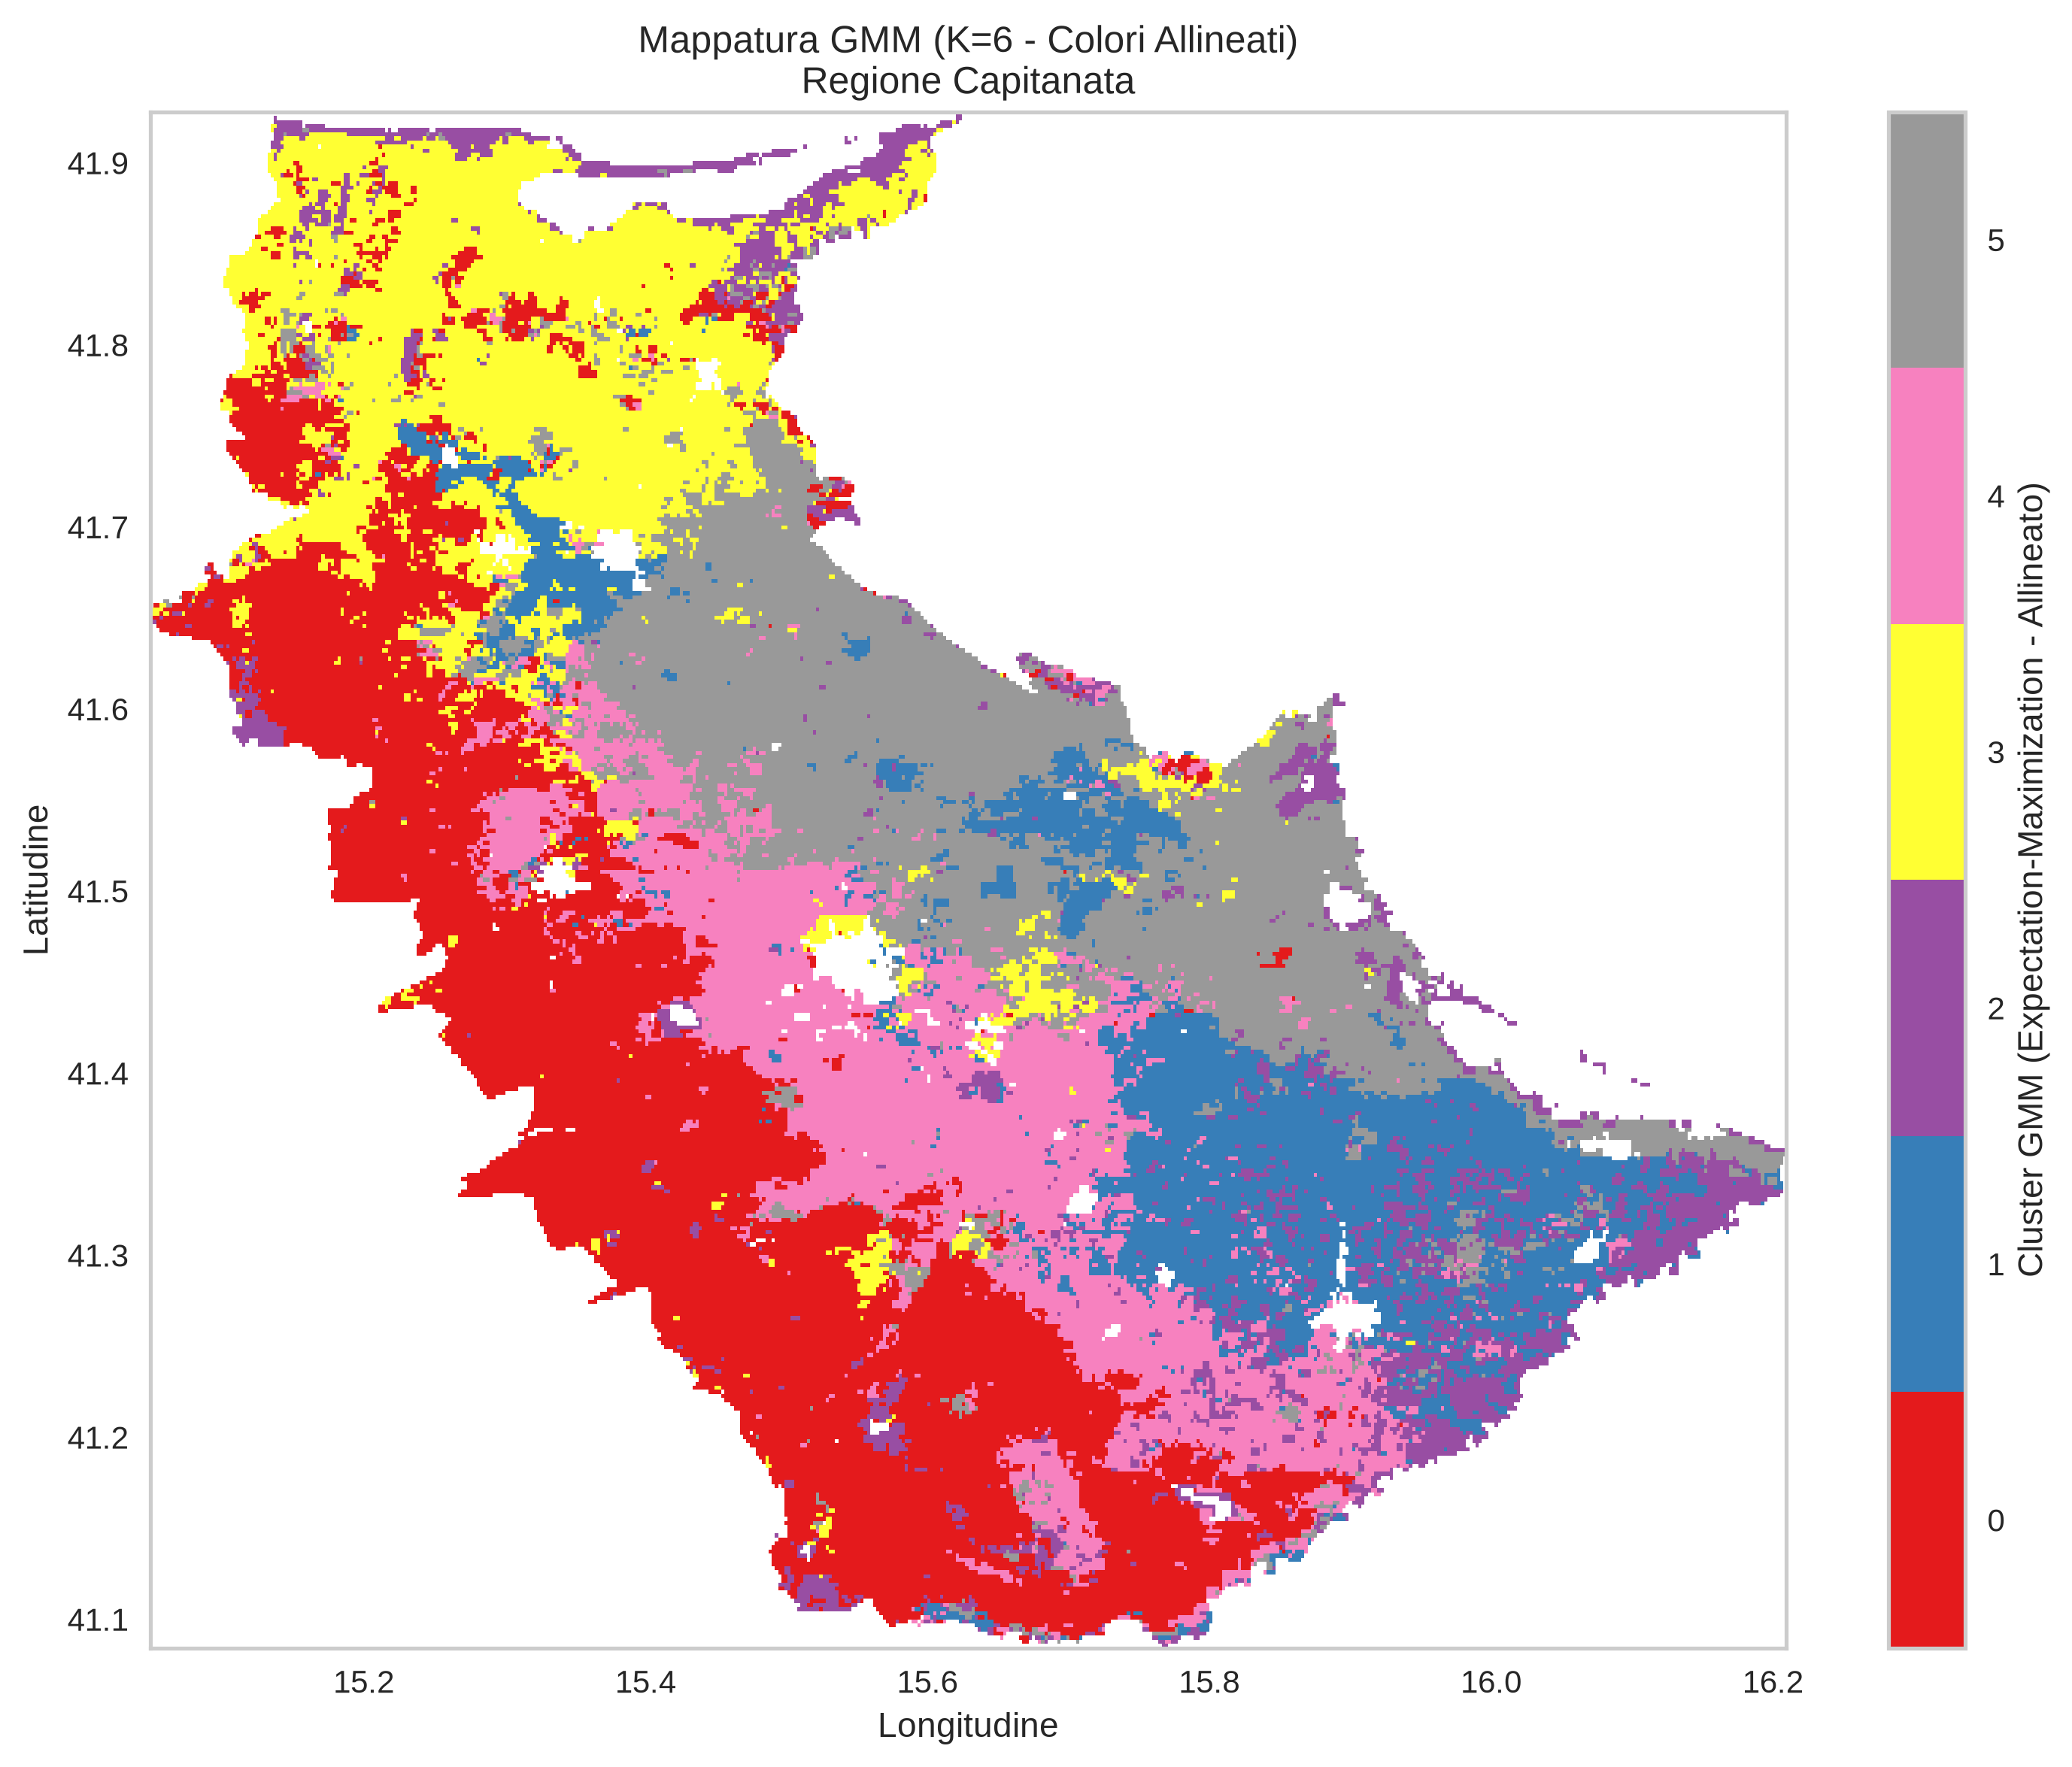
\includegraphics[width=0.8\textwidth]{mappa_gmm.png}
    \caption{Mappatura spaziale dei cluster GMM con \kval{6}.
    L'assegnazione è basata sulla componente gaussiana con
    probabilità a posteriori massima (\emph{hard assignment}).
    Le etichette sono allineate al \kmeans{} per confronto diretto.}
    \label{fig:mappa_gmm}
\end{figure}

\subsection{Validazione e Confronto dei Modelli}

La Tabella~\ref{tab:validazione} riporta il confronto quantitativo tra
i quattro algoritmi. Si noti che per il DBSCAN il Coefficiente di
Silhouette è stato calcolato escludendo i punti di rumore
(cfr.\ Sezione~\ref{sec:metodologia}).

\begin{table}[H]
    \centering
    \caption{Confronto delle metriche di validazione interna ($N = 89\,786$ pixel validi).}
    \label{tab:validazione}
    \begin{tabular}{@{}lcc@{}}
        \toprule
        \textbf{Algoritmo} & \textbf{Silhouette} ($\uparrow$) &
        \textbf{SSE / Inerzia} ($\downarrow$) \\
        \midrule
        K-Means ($K=6$)            & 0.1041  & 762\,167 \\
        Bisecting K-Means ($K=6$)  & 0.0739  & 793\,841 \\
        DBSCAN ($\varepsilon=1.9$) & 0.0869$^*$  & N/A \\
        GMM / EM ($K=6$)           & 0.0658  & N/A$^\dagger$ \\
        \bottomrule
    \end{tabular}

    \vspace{4pt}
    {\footnotesize $^*$Calcolato escludendo i 5\,570 pixel (6.20\%) classificati come rumore ($-1$).}\\
    {\footnotesize $^\dagger$Il GMM ottimizza la log-verosimiglianza (BIC $= 2\,781\,079$, AIC $= 2\,775\,163$), non l'SSE.}
\end{table}

Si evidenzia che, nel dominio del monitoraggio ambientale continuo, valori del Coefficiente di Silhouette compresi tra $0.10$ e $0.20$ sono fisiologici e attesi: il profilo pedologico costituisce un continuum privo di frontiere nette o vuoti euclidei, pertanto la coesione geometrica riflette partizioni a transizione graduale piuttosto che partizioni isolate nello spazio delle fasi, come confermato dall'omogenea estensione orizzontale delle lame nel Silhouette Plot di Yellowbrick.

\subsubsection{Concordanza tra Algoritmi: ARI e NMI}

Per quantificare la concordanza strutturale tra le partizioni prodotte
dai diversi algoritmi, sono stati calcolati l'Adjusted Rand Index (ARI)
e la Normalized Mutual Information (NMI)
(Tabella~\ref{tab:concordanza}).

\begin{table}[H]
    \centering
    \caption{Concordanza tra le partizioni dei diversi algoritmi.}
    \label{tab:concordanza}
    \begin{tabular}{@{}lcc@{}}
        \toprule
        \textbf{Confronto} & \textbf{ARI} & \textbf{NMI} \\
        \midrule
        K-Means vs Bisecting K-Means & 0.458 & 0.546\\
        K-Means vs GMM (EM)          & 0.387 & 0.462 \\
        \bottomrule
    \end{tabular}

    \vspace{4pt}
    {\footnotesize ARI = 1 indica accordo perfetto; NMI = 1 indica massima
    informazione condivisa.}
\end{table}

Un ARI di 0.458 tra \kmeans{} e Bisecting \kmeans{} indica una
concordanza moderata tra le due strategie di partizionamento: le
partizioni condividono buona parte della struttura, ma l'approccio
divisivo top-down produce differenze nella gerarchia di suddivisione.
La concordanza con il GMM (ARI $= 0.387$, NMI $= 0.462$) conferma
che l'assegnazione probabilistica è coerente con quella deterministica,
pur con differenze significative nelle zone di transizione pedologica
(15.3\% dei pixel con probabilità $< 70\%$).

\subsection{Efficienza Computazionale: K-Means vs Mini-Batch K-Means}

Per valutare la scalabilità dell'approccio su dataset geospaziali di
grandi dimensioni, è stato condotto un confronto tra \kmeans{} standard
e \textbf{Mini-Batch \kmeans{}} (Tabella~\ref{tab:efficienza}).

Il Mini-Batch \kmeans{} elabora i dati a blocchi di dimensione fissa
(\texttt{batch\_size} $= 1024$), aggiornando i centroidi in modo
incrementale. Questo approccio riduce drasticamente il tempo di
addestramento con un trade-off minimo in termini di inerzia.

\begin{table}[H]
    \centering
    \caption{Confronto efficienza su 89\,786 pixel della Capitanata.}
    \label{tab:efficienza}
    \begin{tabular}{@{}lcc@{}}
        \toprule
        \textbf{Algoritmo} & \textbf{Tempo (s)} ($\downarrow$) &
        \textbf{Inerzia} ($\downarrow$) \\
        \midrule
        K-Means Standard     & 0.437 & 762\,167 \\
        Mini-Batch K-Means   & 0.141 & 780\,138 \\
        \bottomrule
    \end{tabular}
\end{table}

Il Mini-Batch \kmeans{} ha dimostrato un'accelerazione di circa $3\times$
rispetto al \kmeans{} standard, con un incremento dell'inerzia
di circa il 2.4\% (da 762\,167 a 780\,138), confermando la sua idoneità
per applicazioni geospaziali su larga scala.


% ══════════════════════════════════════════════════════════════════════════
\section{Discussione e Conclusioni}
\label{sec:conclusioni}
% ══════════════════════════════════════════════════════════════════════════

\subsection{Sintesi dei Risultati}

Il lavoro ha dimostrato che l'approccio basato sui \textbf{gradienti
verticali} consente di superare i limiti del clustering bidimensionale,
catturando informazioni sulla struttura tridimensionale del profilo
pedologico. I principali risultati sono:

\begin{enumerate}
    \item La \textbf{feature engineering} basata su 13
    gradienti normalizzati si è dimostrata efficace nel catturare le
    dinamiche verticali del suolo, producendo cluster con
    interpretazione agronomica chiara. L'analisi di correlazione ha
    confermato l'assenza di collinearità critica tra le feature.

    \item Il \textbf{\kmeans{}} con \kval{6} ha prodotto la migliore
    separazione spaziale, con cluster geograficamente coerenti con la
    geomorfologia della Capitanata. La scelta di $K$ è stata supportata
    dal Metodo del Gomito, dall'Indice di Davies-Bouldin e da
    considerazioni agronomiche di dominio.

    \item Il \textbf{DBSCAN} ha classificato una porzione significativa
    di pixel come rumore, confermando che la distribuzione dei dati nello
    spazio dei gradienti non è caratterizzata da cluster a densità
    nettamente diversa, ma piuttosto da regioni a densità omogenea
    (scenario favorevole al \kmeans{}).

    \item Il \textbf{Bisecting \kmeans{}} ha fornito risultati
    con concordanza moderata rispetto al \kmeans{} standard
    (ARI $= 0.458$), indicando che l'approccio divisivo top-down
    converge verso una struttura simile ma non identica, con
    differenze nella gerarchia di suddivisione.

    \item Il \textbf{GMM} (algoritmo EM) ha offerto un'assegnazione
    probabilistica dei pixel ai cluster, evidenziando le zone di
    transizione pedologica con incertezza elevata (pixel con probabilità
    $< 70\%$). La selezione del modello tramite BIC e AIC ha confermato
    la ragionevolezza della scelta $K=6$. I cluster GMM mostrano una
    struttura spaziale comparabile a quella del \kmeans{}, con confini
    leggermente più sfumati dovuti alla natura ellissoidale delle
    componenti gaussiane.

    \item Il \textbf{Mini-Batch \kmeans{}} ha confermato la scalabilità
    dell'approccio a dataset geospaziali di grandi dimensioni, con
    un'accelerazione di circa $3\times$ (0.141\,s vs 0.437\,s) e un
    incremento dell'inerzia limitato al 2.4\%.
\end{enumerate}

\subsection{Limiti dello Studio}

\begin{itemize}
    \item \textbf{Assenza di ground-truth}: trattandosi di clustering
    non supervisionato, non è possibile calcolare metriche esterne
    basate su etichette reali. La validazione si basa su indici
    interni (Silhouette, SSE, DB, CH), concordanza tra algoritmi
    (ARI, NMI) e coerenza spaziale.

    \item \textbf{Risoluzione spaziale}: la griglia SoilGrids a
    250\,m media le proprietà su pixel relativamente grandi, potendo
    mascherare variabilità locale.

    \item \textbf{Scelta di $K$}: la scelta di $K=6$ è stata guidata
    da un bilanciamento tra metriche statistiche e conoscenze di dominio
    agronomico, ma potrebbe beneficiare di una validazione con dati
    di campo (profili pedologici reali).
\end{itemize}

\subsection{Sviluppi Futuri}

Possibili estensioni del lavoro includono:

\begin{itemize}
    \item L'integrazione di \textbf{dati climatici e morfologici}
    (precipitazioni, pendenza, uso del suolo) come feature aggiuntive.

    \item L'applicazione di algoritmi di clustering
    \textbf{spazialmente vincolati} che incorporino la prossimità
    geografica nel calcolo delle distanze.

    \item L'estensione dell'analisi all'\textbf{intera regione Puglia}
    o al Sud Italia per validare la generalizzabilità dell'approccio.

    \item L'impiego di tecniche di \textbf{deep clustering}
    (autoencoders + clustering nello spazio latente) per catturare
    relazioni non lineari tra le feature.
\end{itemize}

\end{document}
